\documentclass[12pt]{article}
\usepackage[utf8]{inputenc}
\usepackage[a4paper, total={6.5in, 9.5in}]{geometry}
\usepackage{authblk}
\usepackage{multirow}
\usepackage{graphicx}
\usepackage{amsmath}
\usepackage{biblatex}
\usepackage{rotating}
\usepackage{ragged2e}
\usepackage{multicol}
\usepackage{float}
\usepackage{algpseudocode}
\usepackage{enumitem}
\usepackage{caption}
\usepackage{subcaption}
\usepackage{hyperref}
\hypersetup{
    colorlinks=true,
    linkcolor=blue,
    }
\usepackage[label=corner]{karnaugh-map}
\usepackage[siunitx, RPvoltages]{circuitikz}
\usetikzlibrary{calc}
\usepackage{tikz}
\usetikzlibrary{positioning, shapes, arrows.meta, calc}

\begin{document}
\newpage

\section{\large{Description and Circuit Diagram of Important Blocks}}
Some libraries and circuits were implemented to enhance and simplify the final circuit design.Those are :

\subsection{Multiplexer Library}
The modular circuits in this library are as follows 
\begin{itemize}

    \item 11 bit 2 to 1 Mux 
    \item 12 bit 2 to 1 Mux 
    \item 32 bit 2 to 1 Mux 

\end{itemize}
\begin{figure}[H]
    \centering
    \begin{subfigure}[b]{0.3\textwidth}
        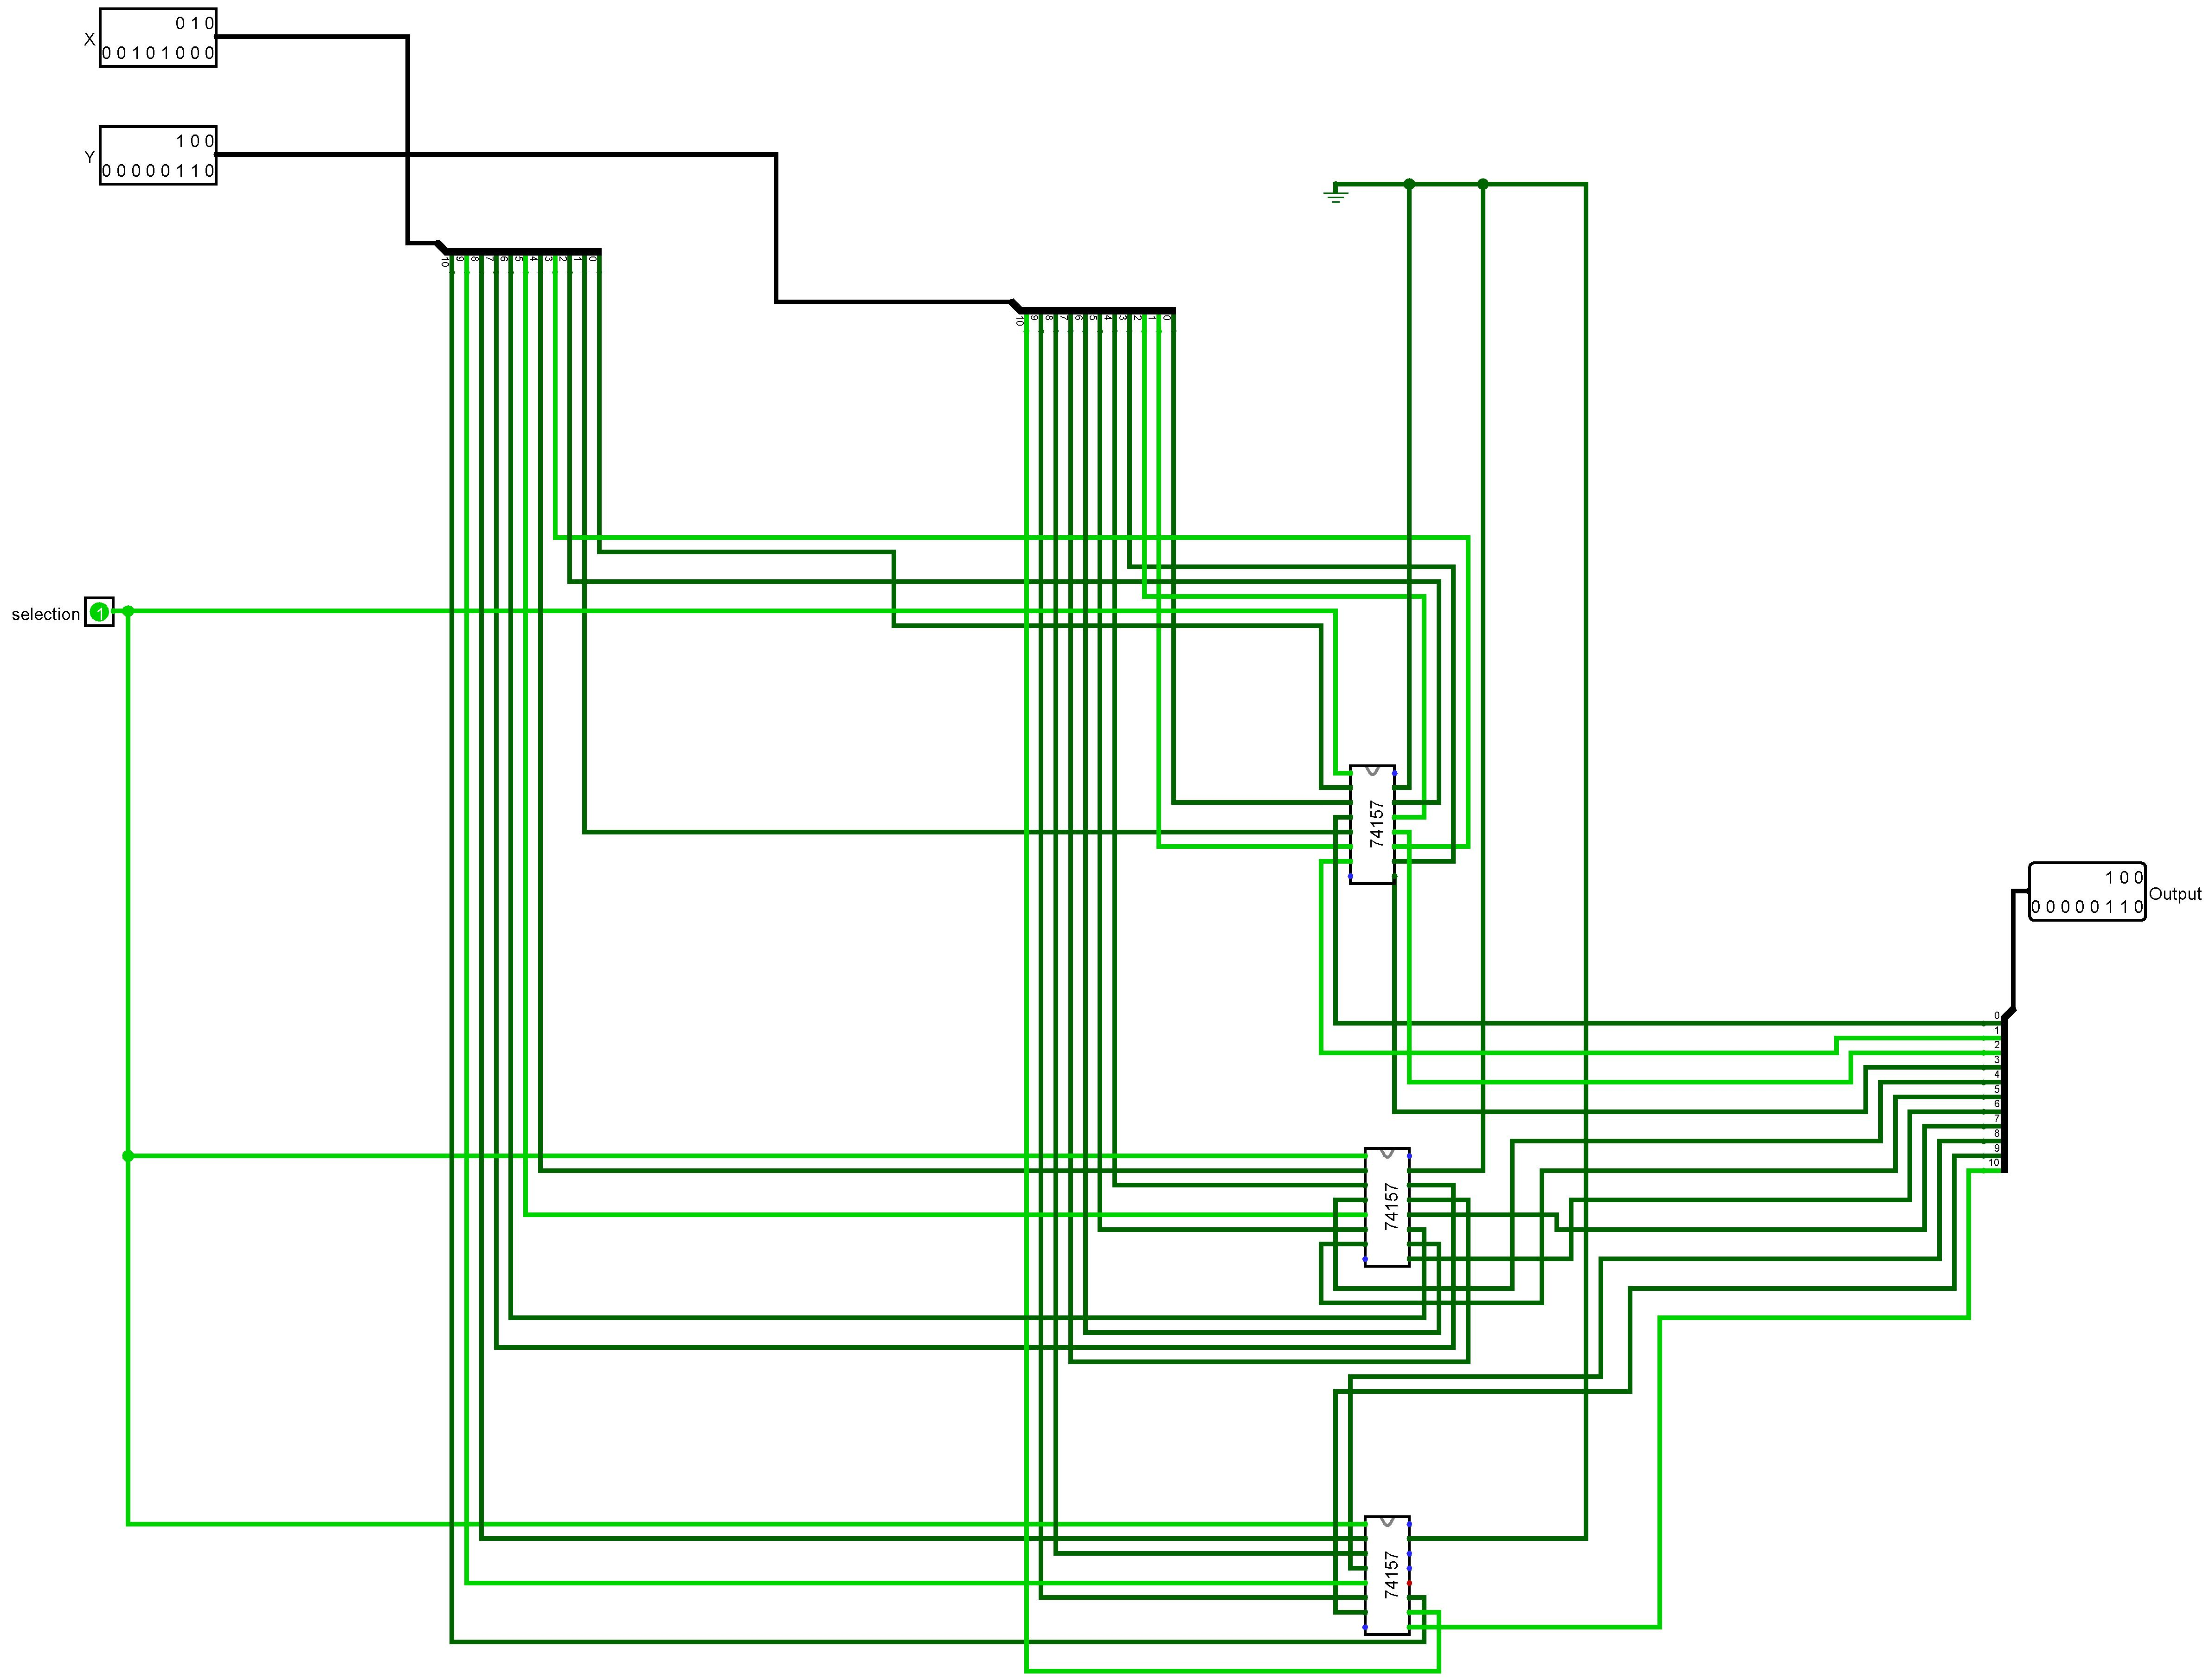
\includegraphics[width=\textwidth]{MUX_11_bit.jpg}
        \caption{11 bit $2\times1$ MUX}
        \label{fig:11b2x1mux}
    \end{subfigure}
    \begin{subfigure}[b]{0.3\textwidth}
        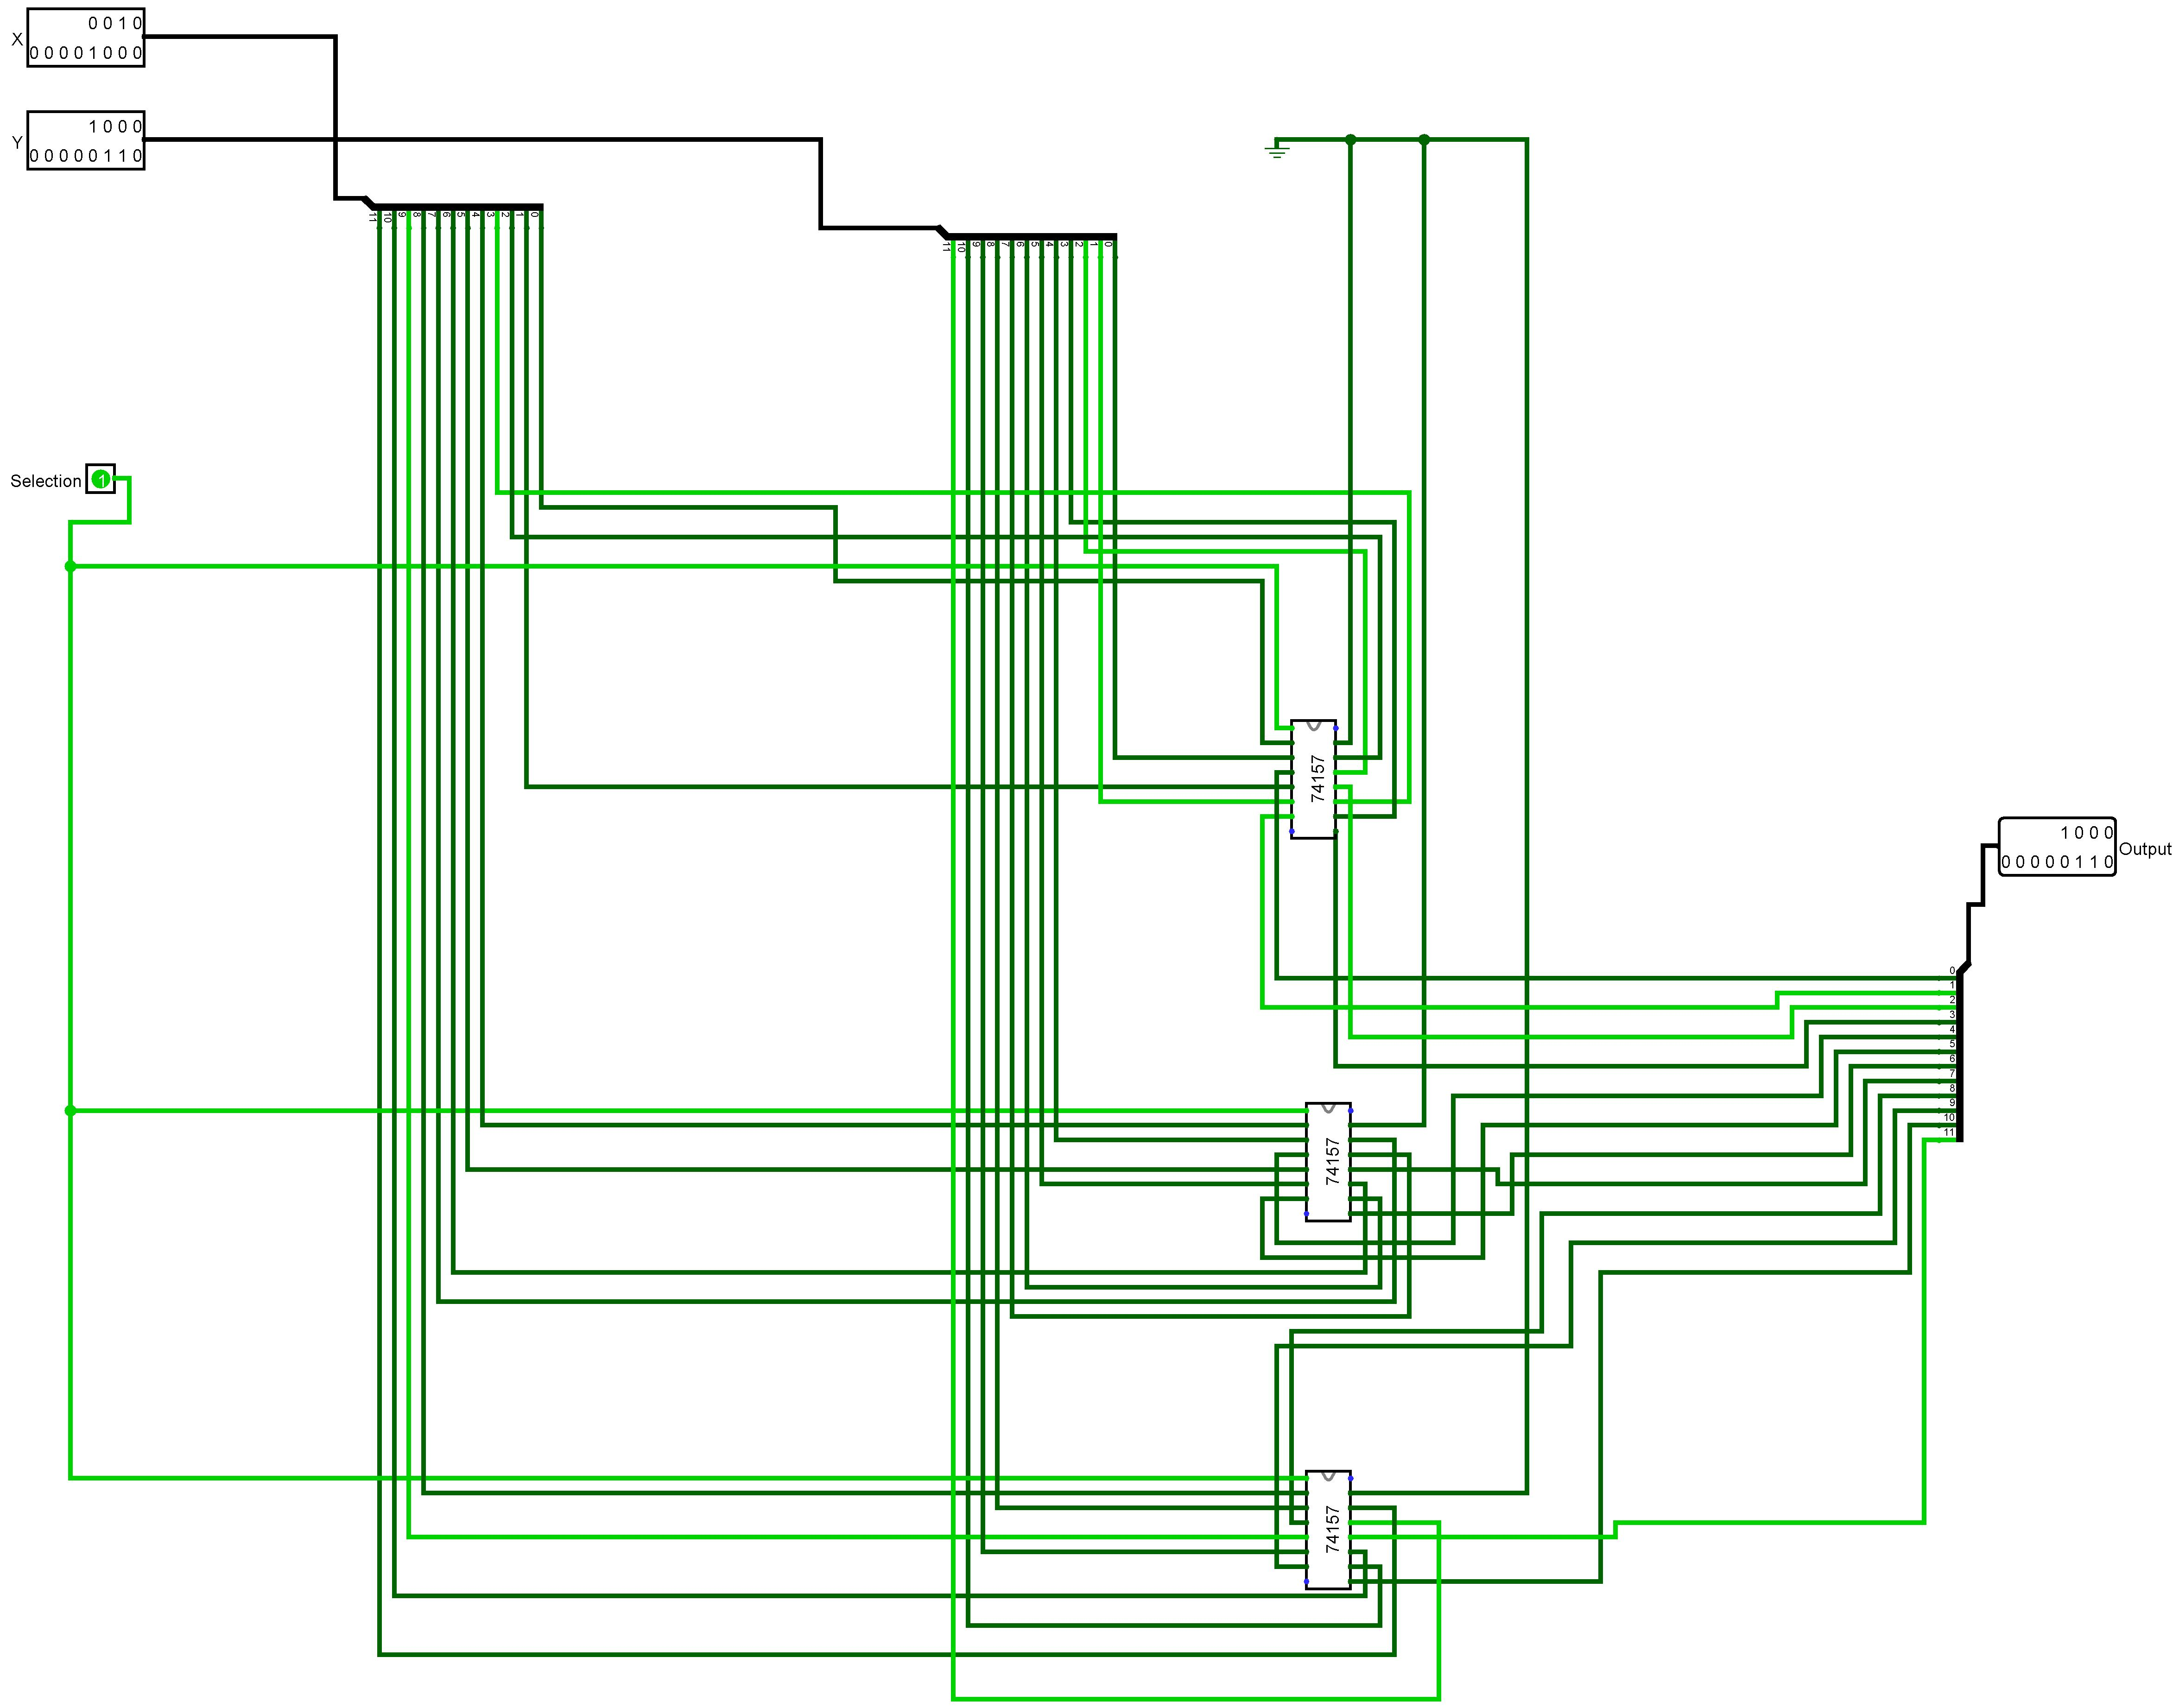
\includegraphics[width=\textwidth]{MUX_12_bit.jpg}
        \caption{12 bit $2\times1$ MUX}
        \label{fig:12b2x1mux}
    \end{subfigure}
     \newline
     \newline
    \begin{subfigure}[b]{0.4\textwidth}
        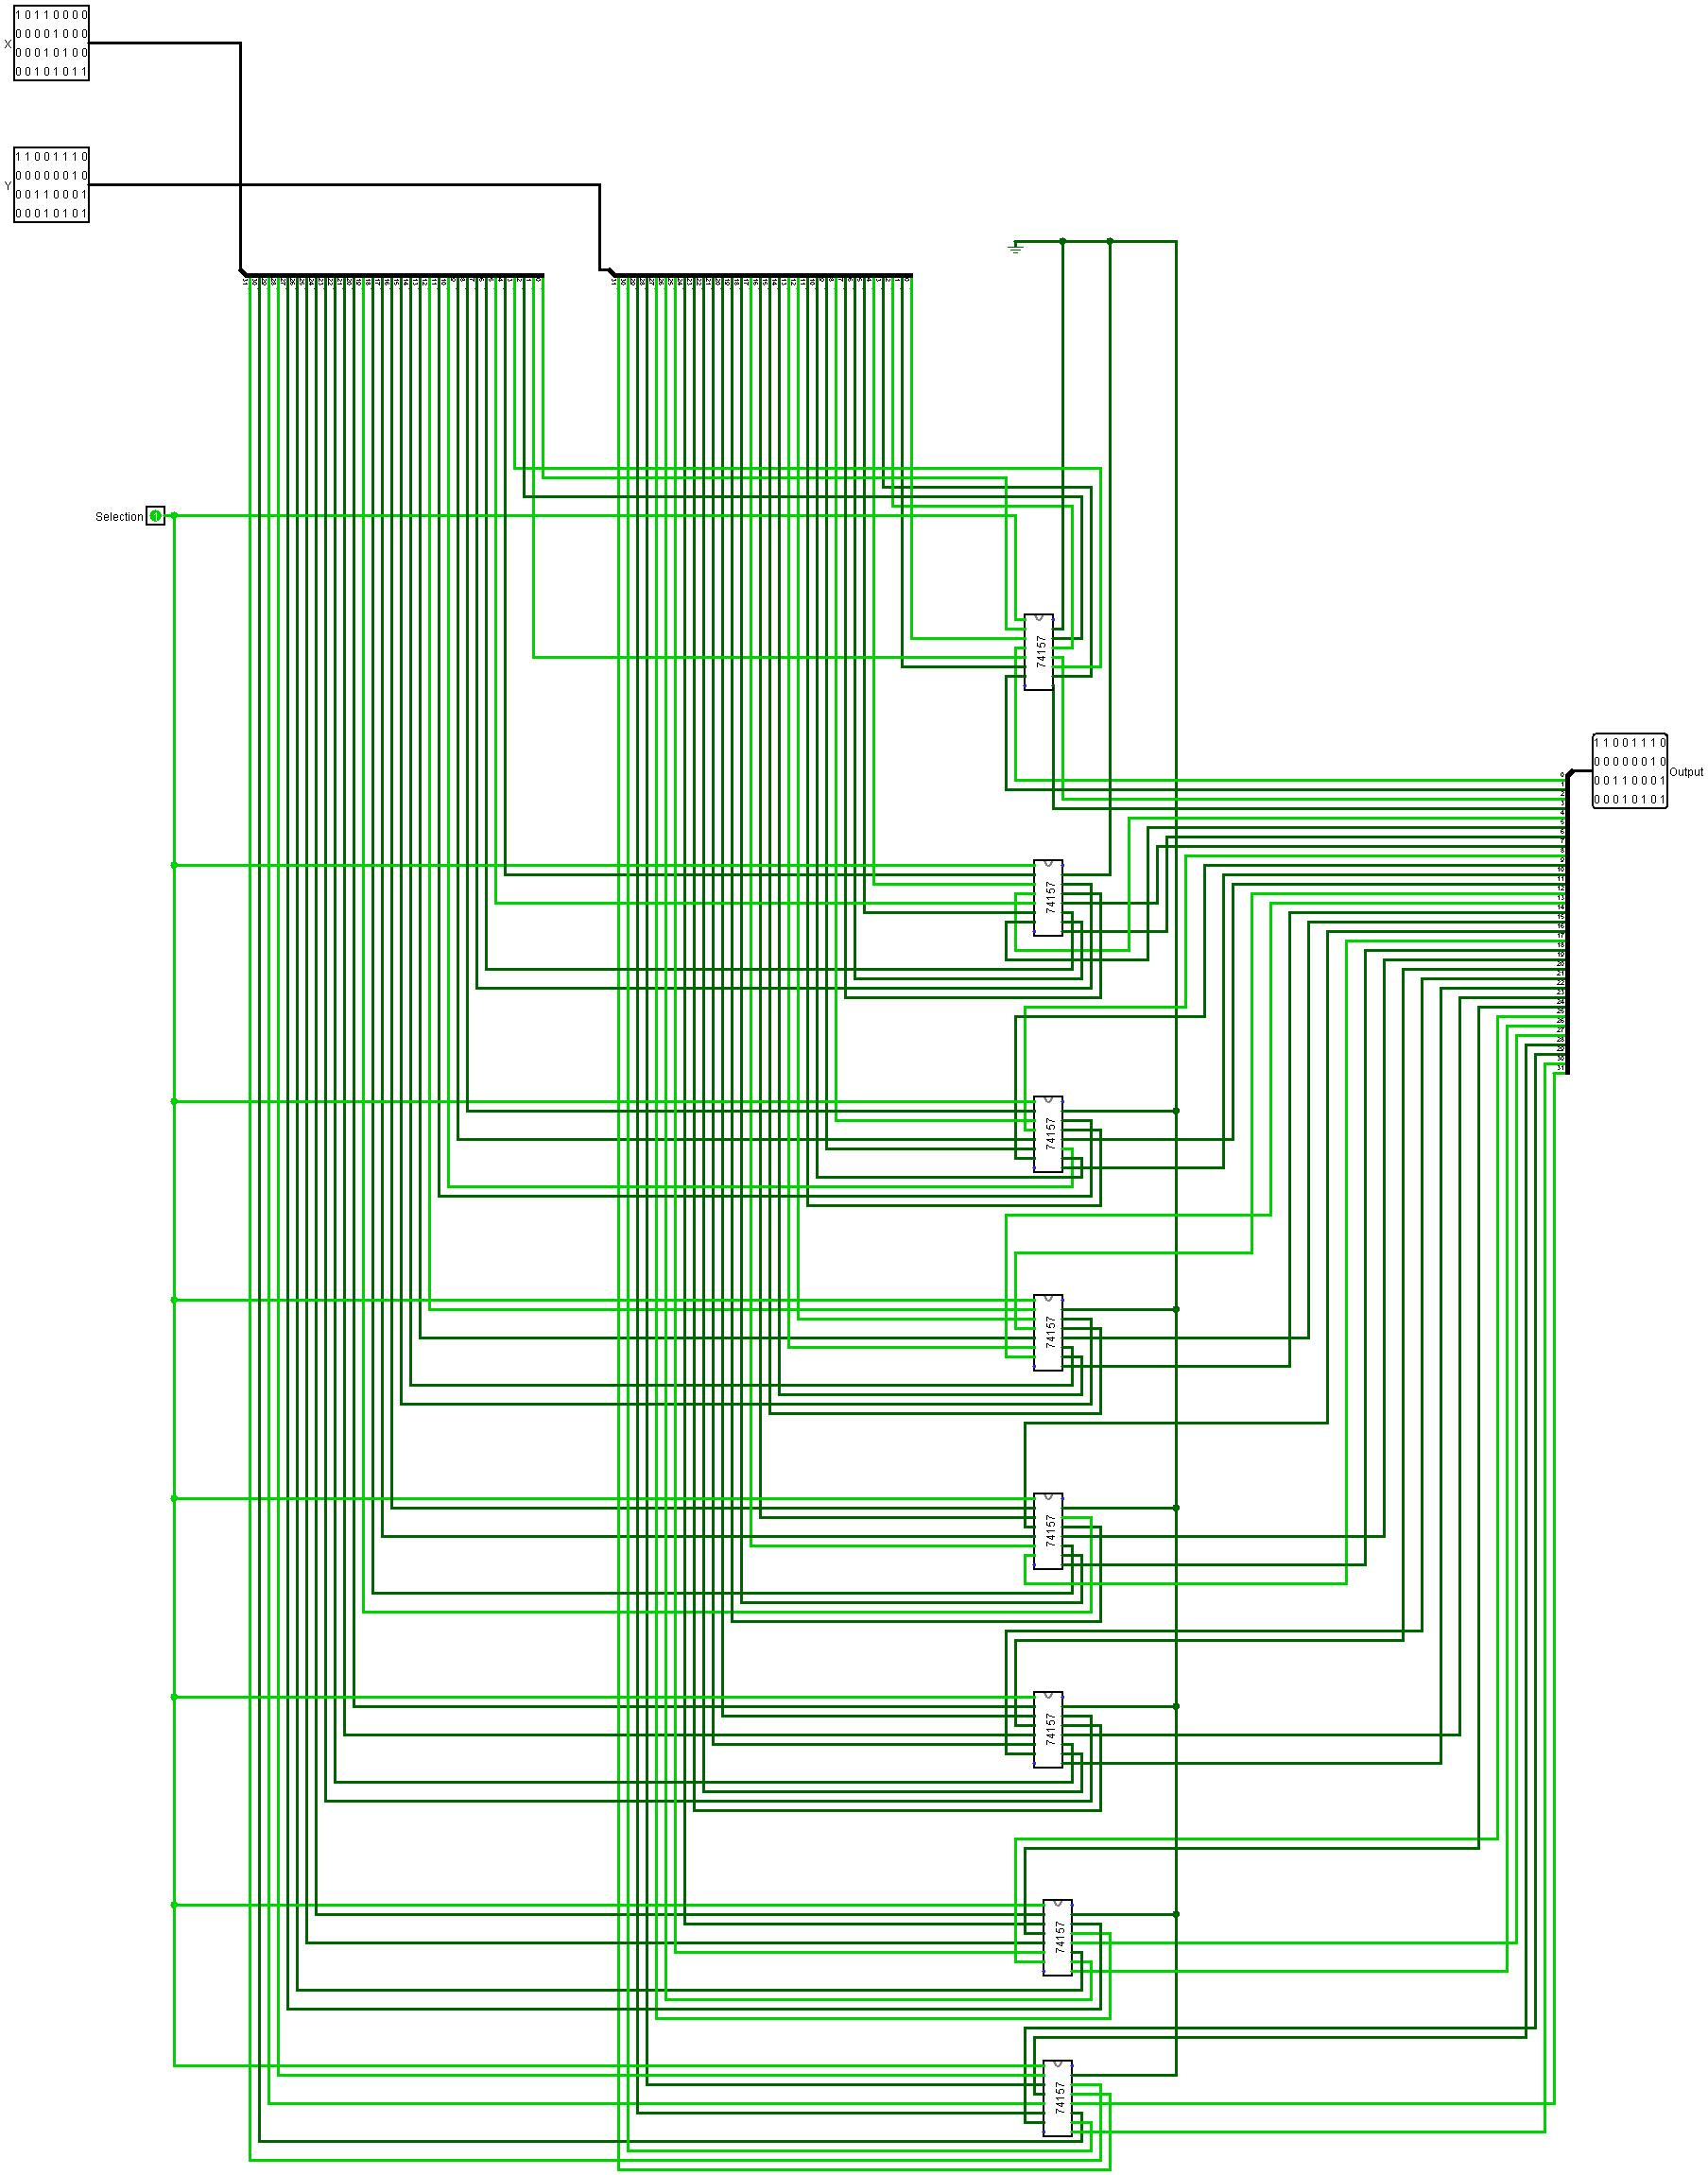
\includegraphics[width=\textwidth]{MUX_32_bit.jpg}
        \caption{32 bit $2\times1$ MUX}
        \label{fig:32b2x1}
    \end{subfigure}

    \caption{Multiplexer Circuits}\label{fig:mux}
\end{figure}

\newpage

\subsection{Comparator Library}
An comparator library was constructed to compare the exponenets . This library contains 2 circuits i.e. an 11 bit magnitude comparator and a comparator for small fractions.
\begin{figure}[H]
    \centering
    \begin{subfigure}{\textwidth}
    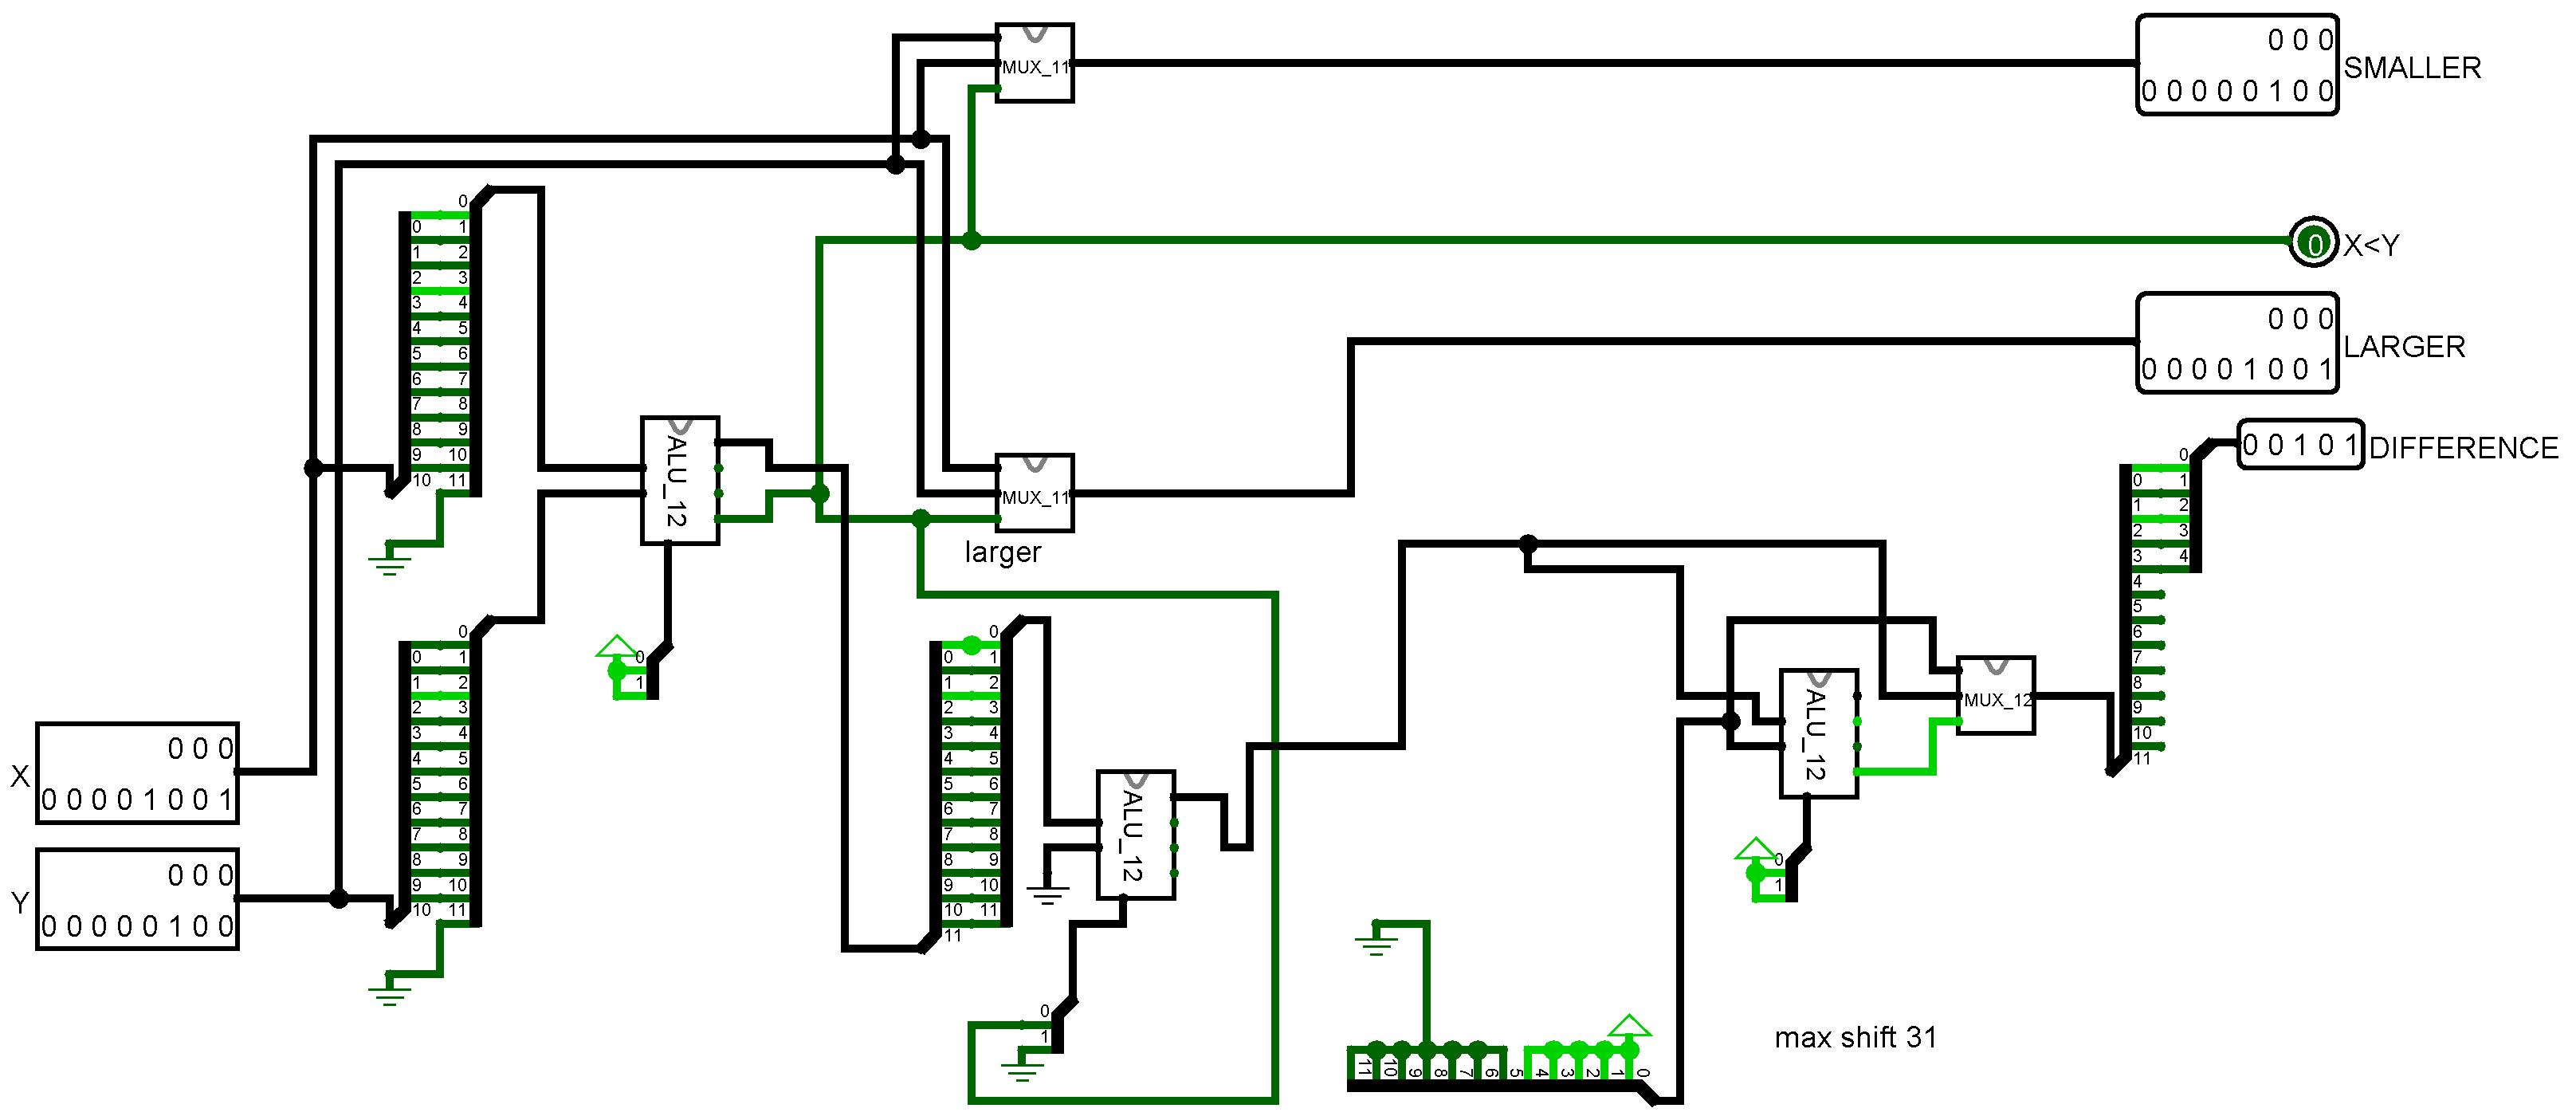
\includegraphics[width=\textwidth]
        {Comparator_11_bit.jpg}
        \label{fig:11bitmagcomp}
    \caption{11 Bit Magnitude Comparator}
        
    \end{subfigure}
    \begin{subfigure}{\textwidth}
    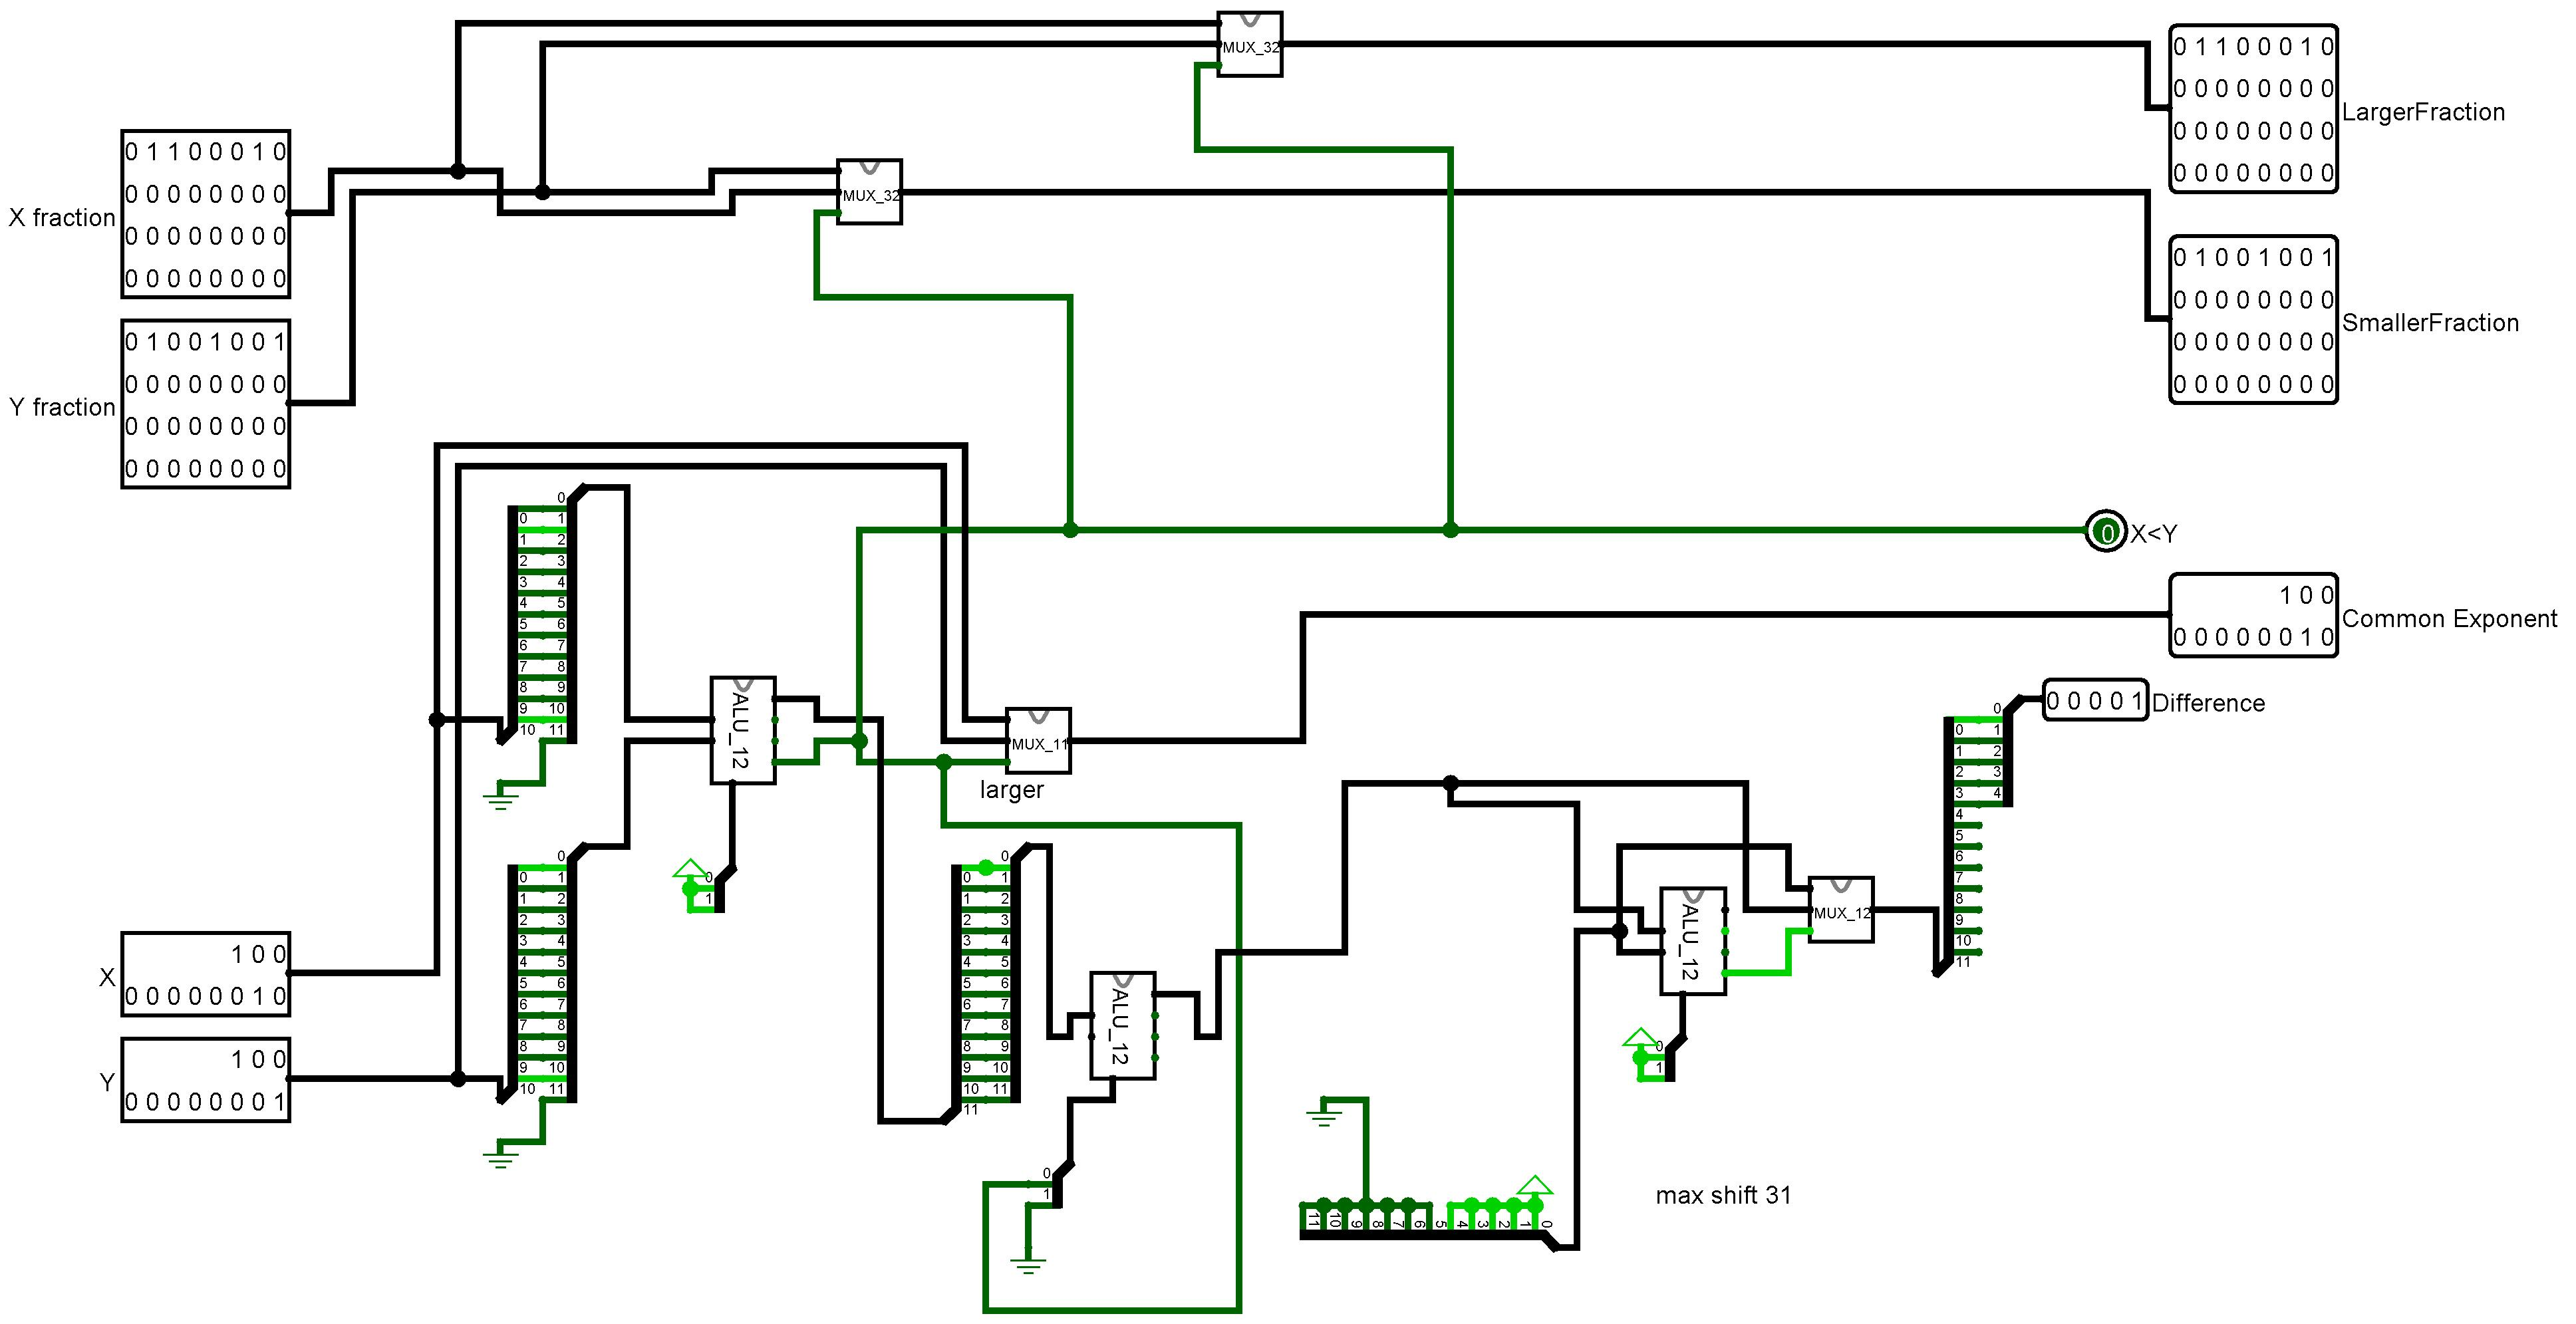
\includegraphics[width=\textwidth]
        {Comparator_With_Smaller_Fraction.jpg}
        \label{fig:smfracmagcomp}
    \caption{Smaller Fractions Magnitude Comparator}
        
    \end{subfigure}
    \label{fig:magcomps}
    \caption{Magnitude Comparators}
        
\end{figure}
\newpage
\subsection{Adder-Subtractor Library}
A 32 bit adder-subtractor circuit was implemented to add or subtract 2 signed numbers
\begin{figure}[H]
    \centering
        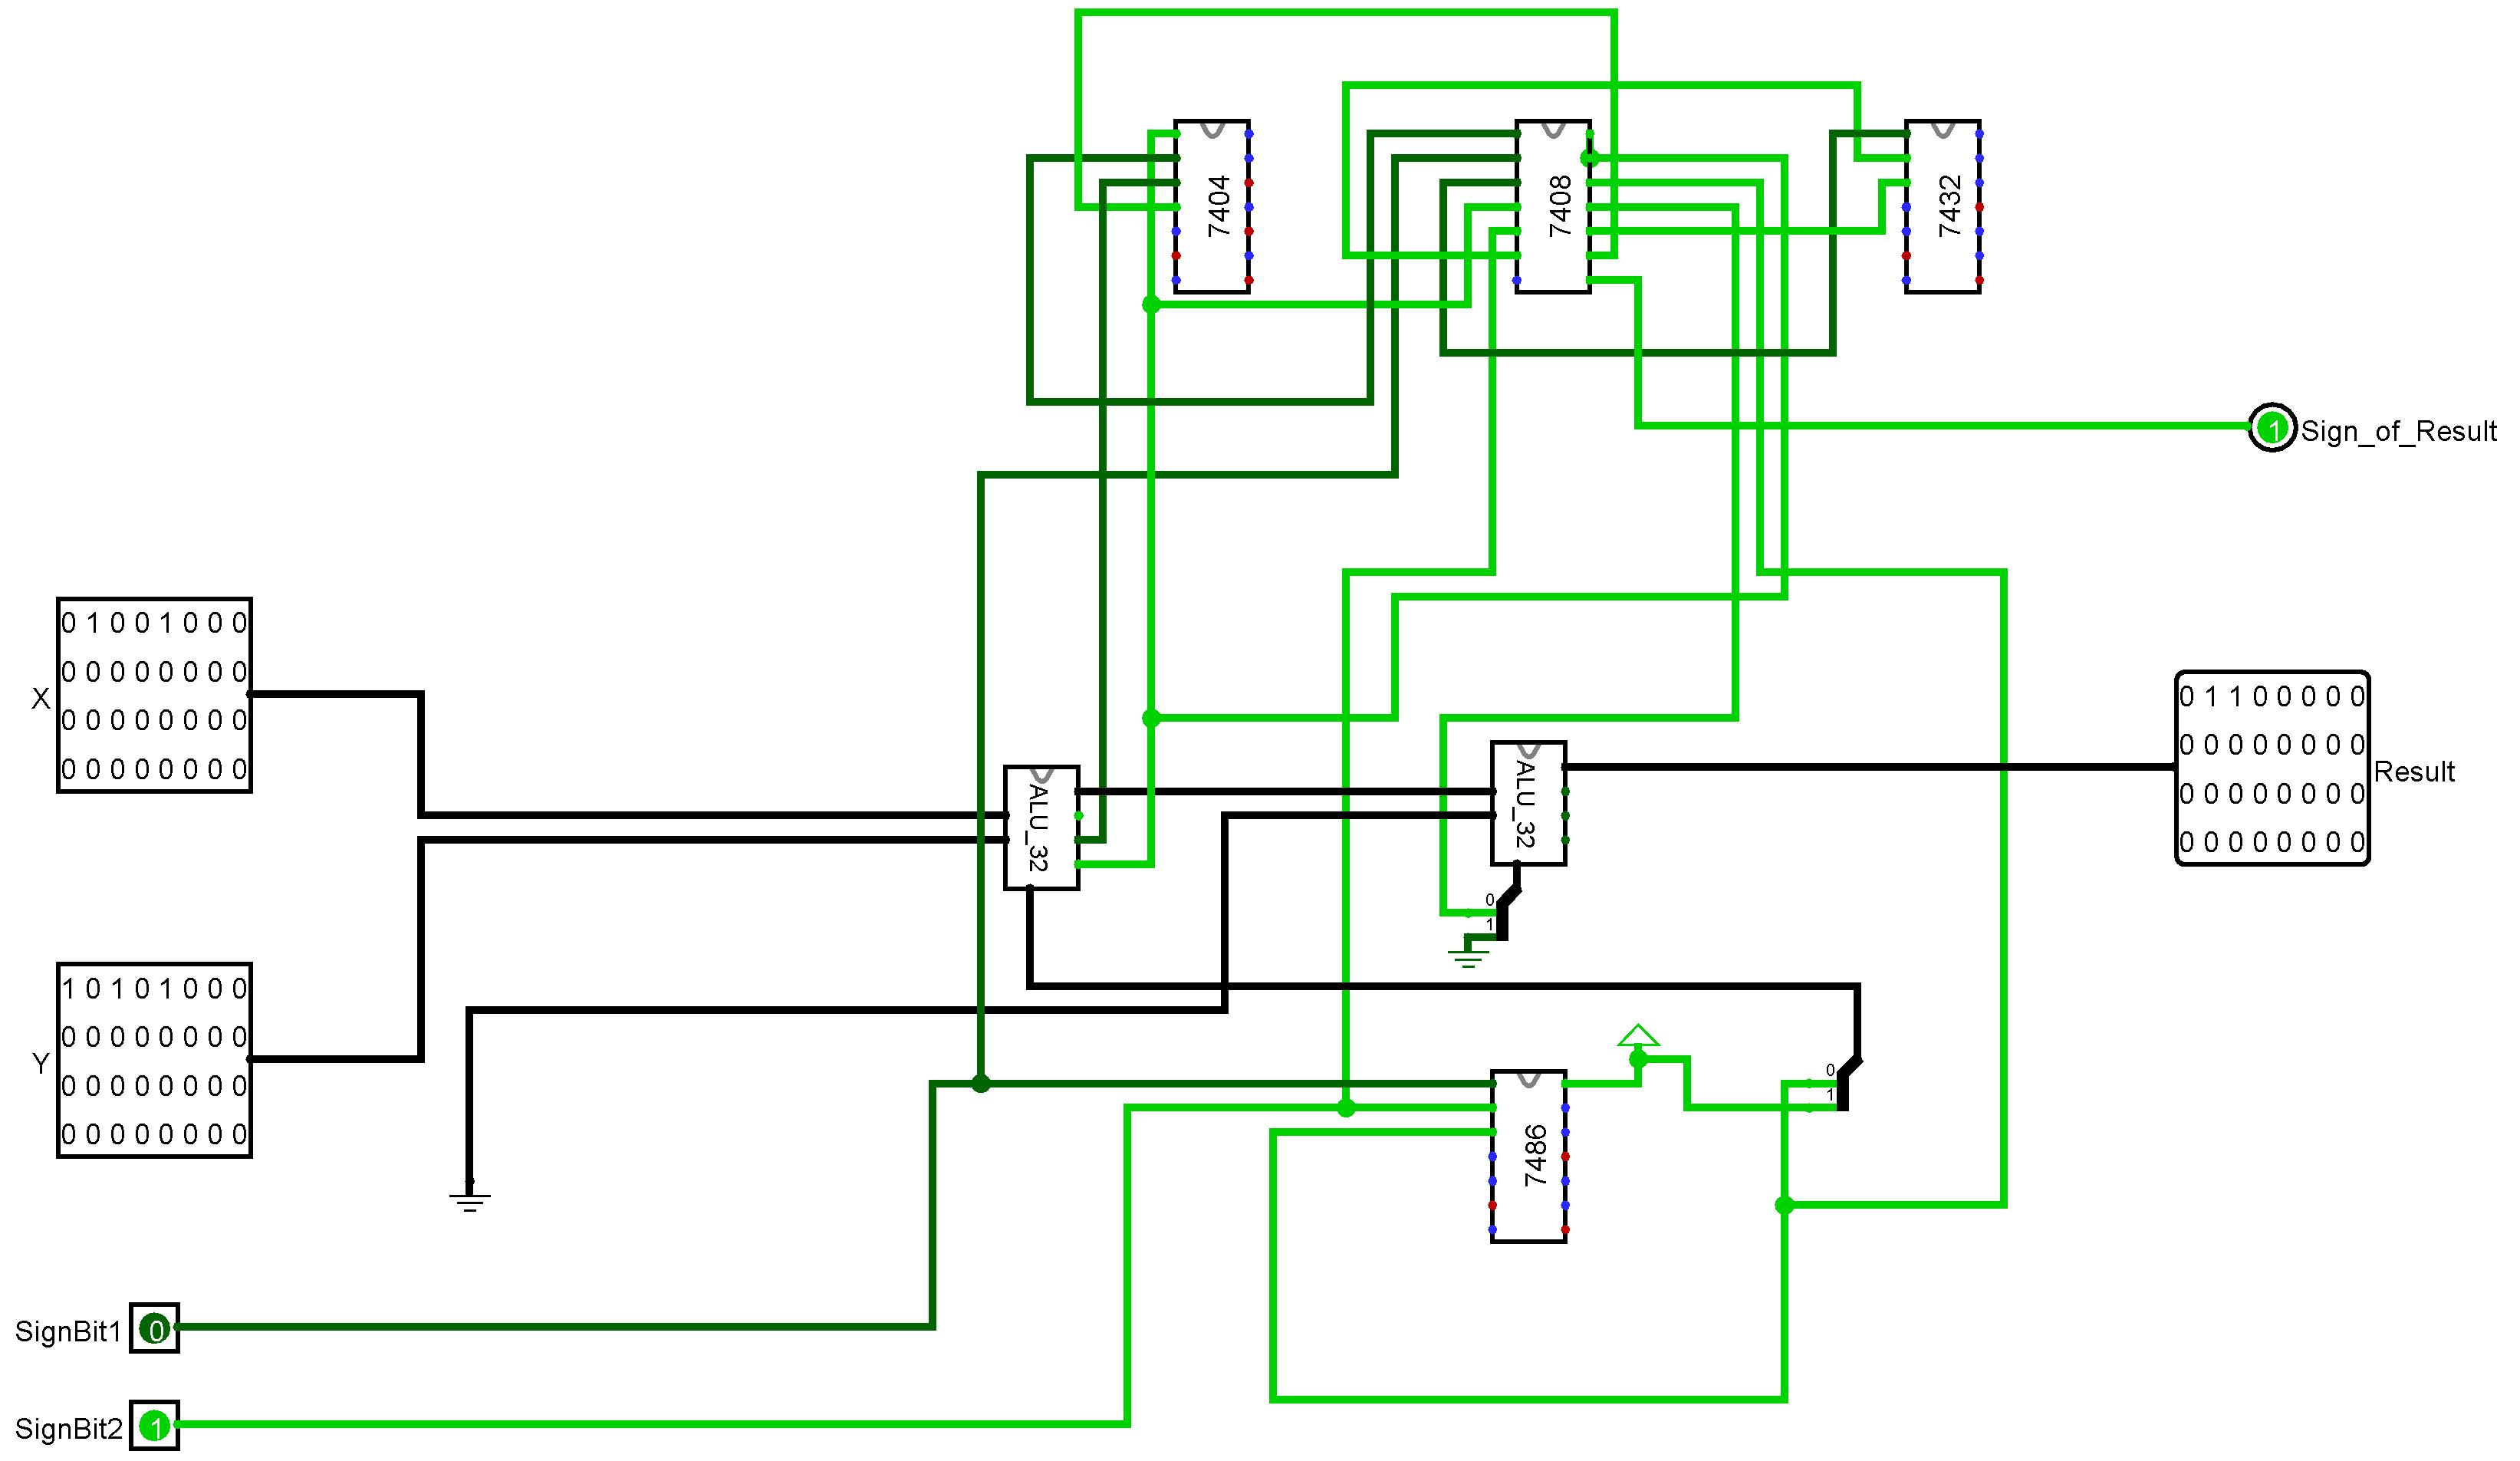
\includegraphics[width=\textwidth]{Adder_Subtractor.jpg}
        \caption{32 bit Adder$-$Subtractor}
        \label{fig:32bitaddsub}
\end{figure}

\newpage
\subsection{Encoder Library}
To normalize a number, we need to locate the first set bit starting from MSB. 3 priority encoders was used for this purpose. Those are :
\begin{itemize}
    \item 8 to 3 priority encoder 
    \item 16 to 4 priority encoder 
    \item 32 to 5 priority encoder 
\end{itemize}
\begin{figure}[H]
    \centering
    \begin{subfigure}[b]{0.45\textwidth}
        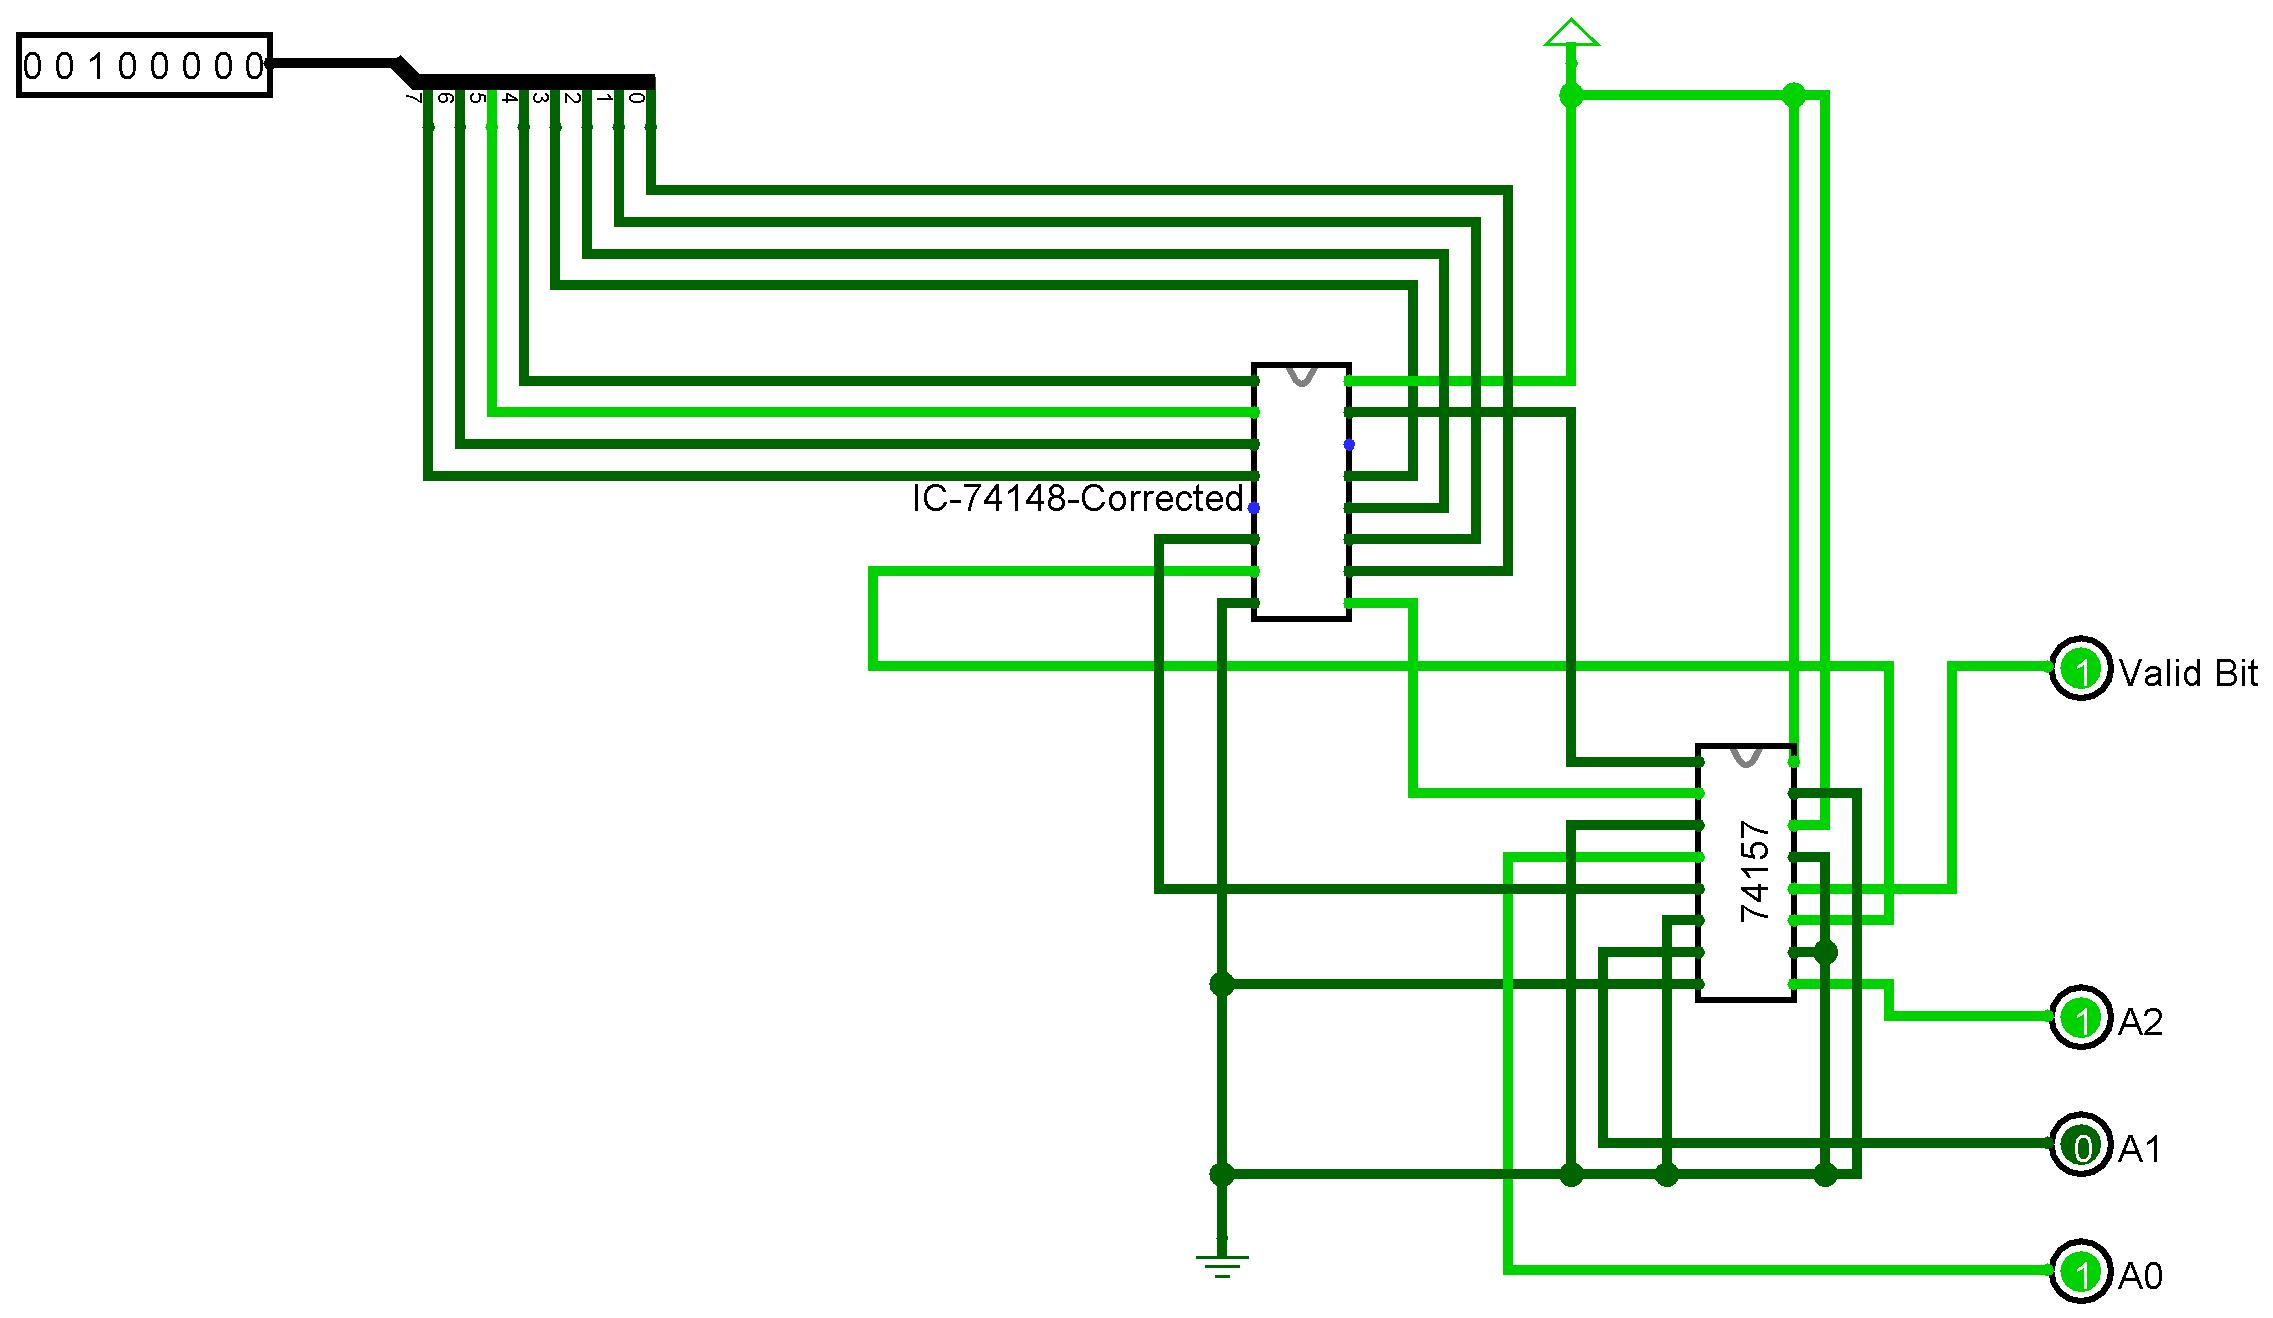
\includegraphics[width=\textwidth]{PE_8x3.jpg}
        \caption{8$\times$3 Priority Encoder}
        \label{fig:8x3prioenc}
    \end{subfigure}
    \begin{subfigure}[b]{0.45\textwidth}
        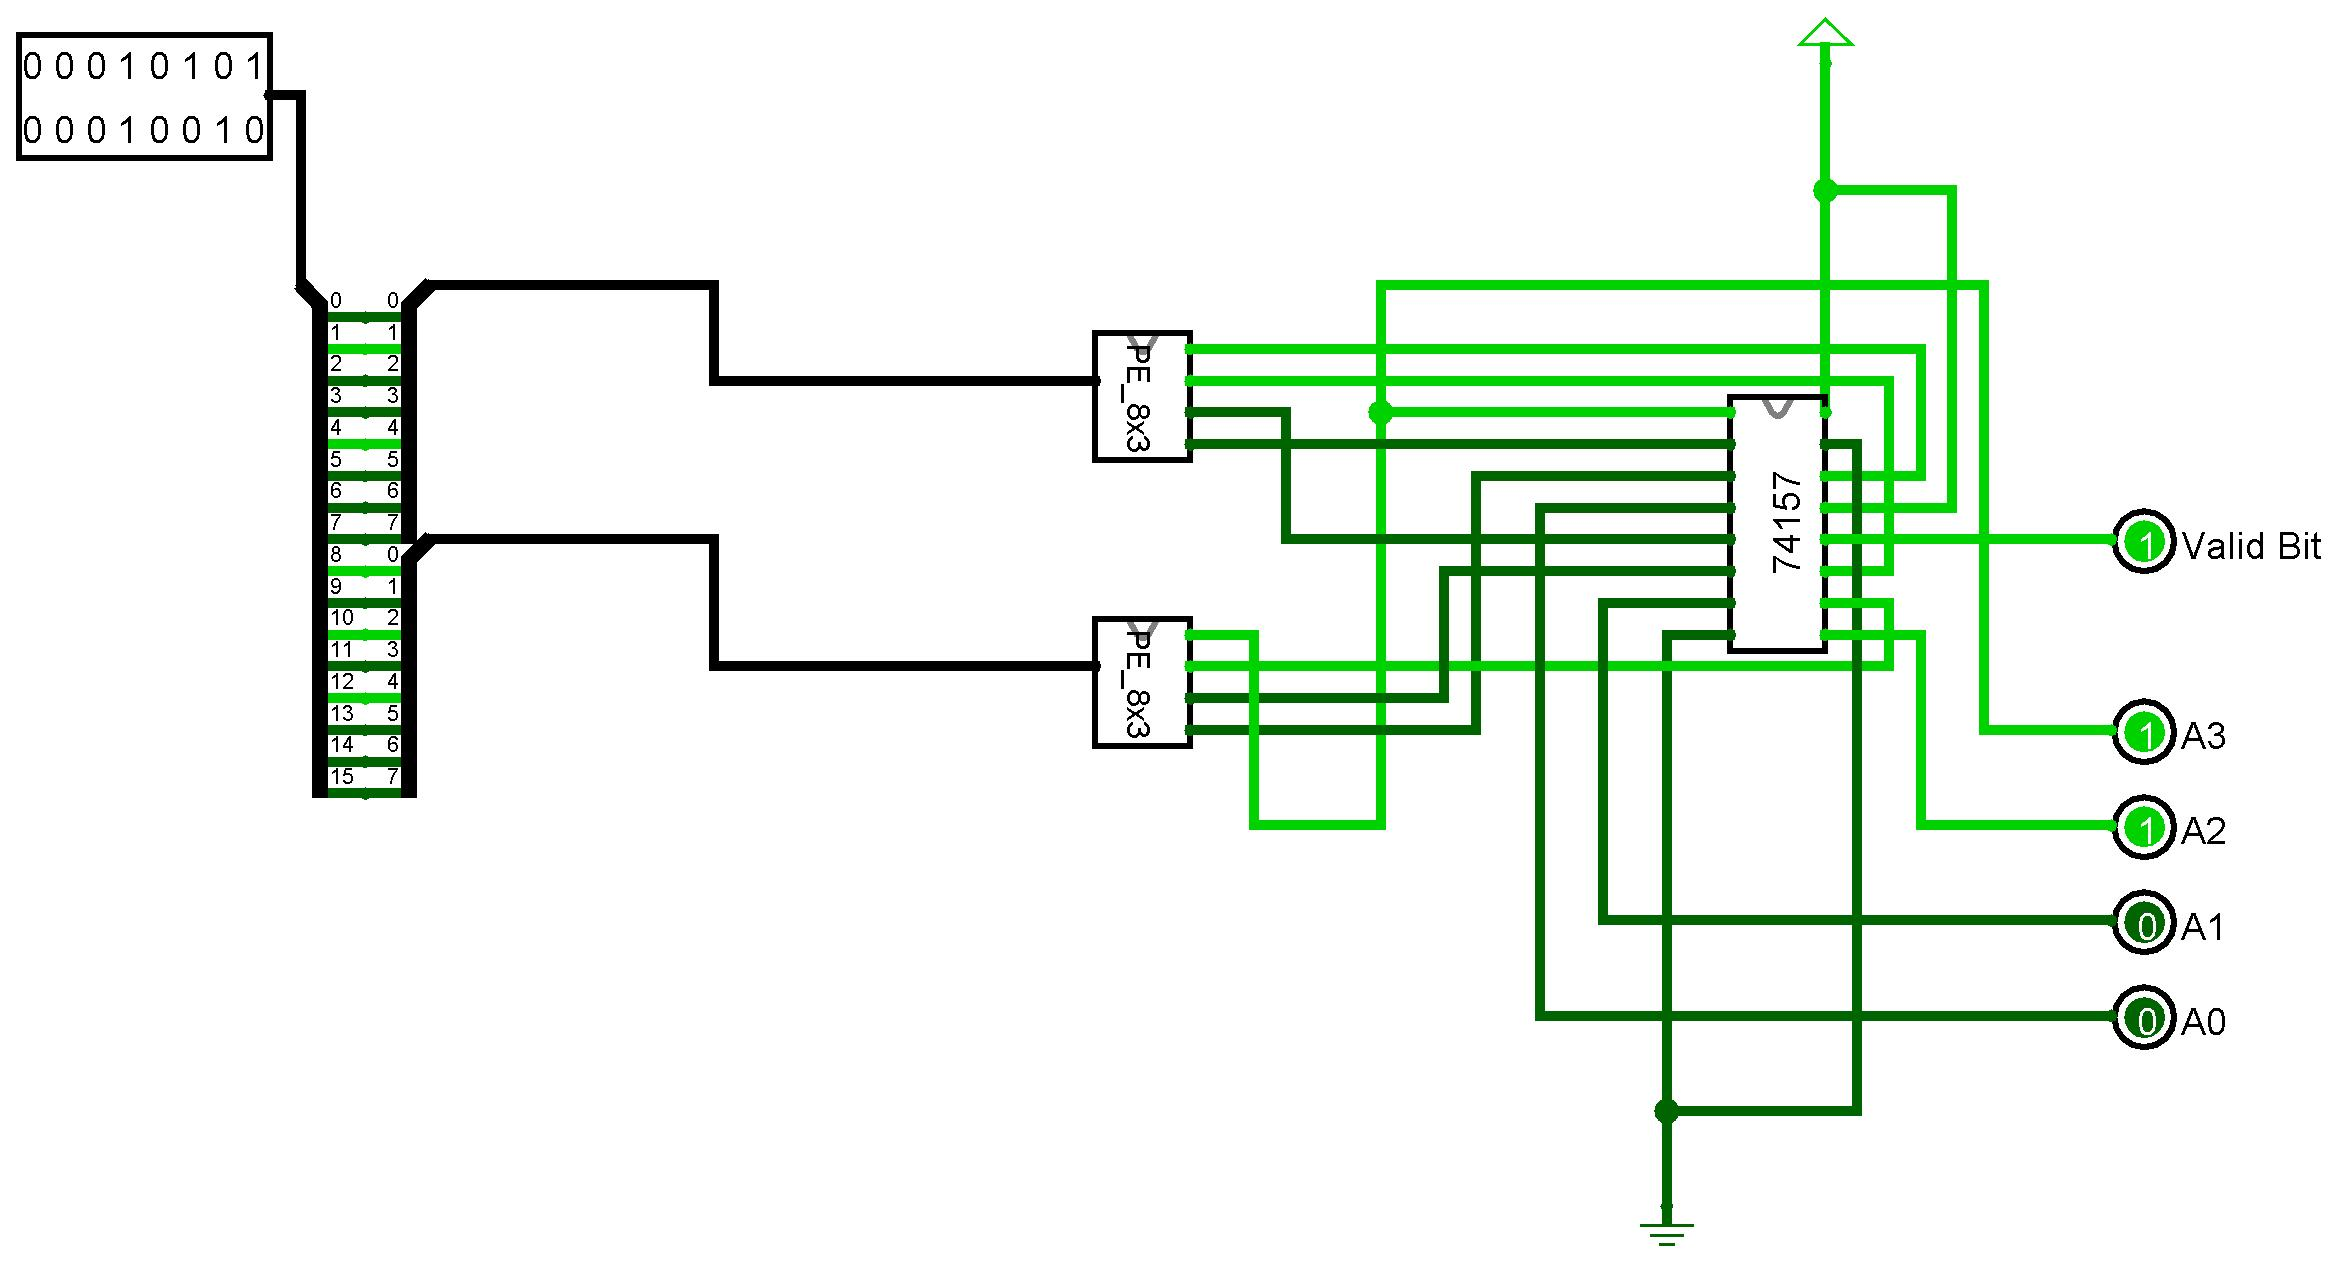
\includegraphics[width=\textwidth]{PE_16x4.jpg}
        \caption{16$\times$4 Priority Encoder}
        \label{fig:16x4prioenc}
    \end{subfigure}
    \newline
    \newline
    \begin{subfigure}[b]{0.9\textwidth}
        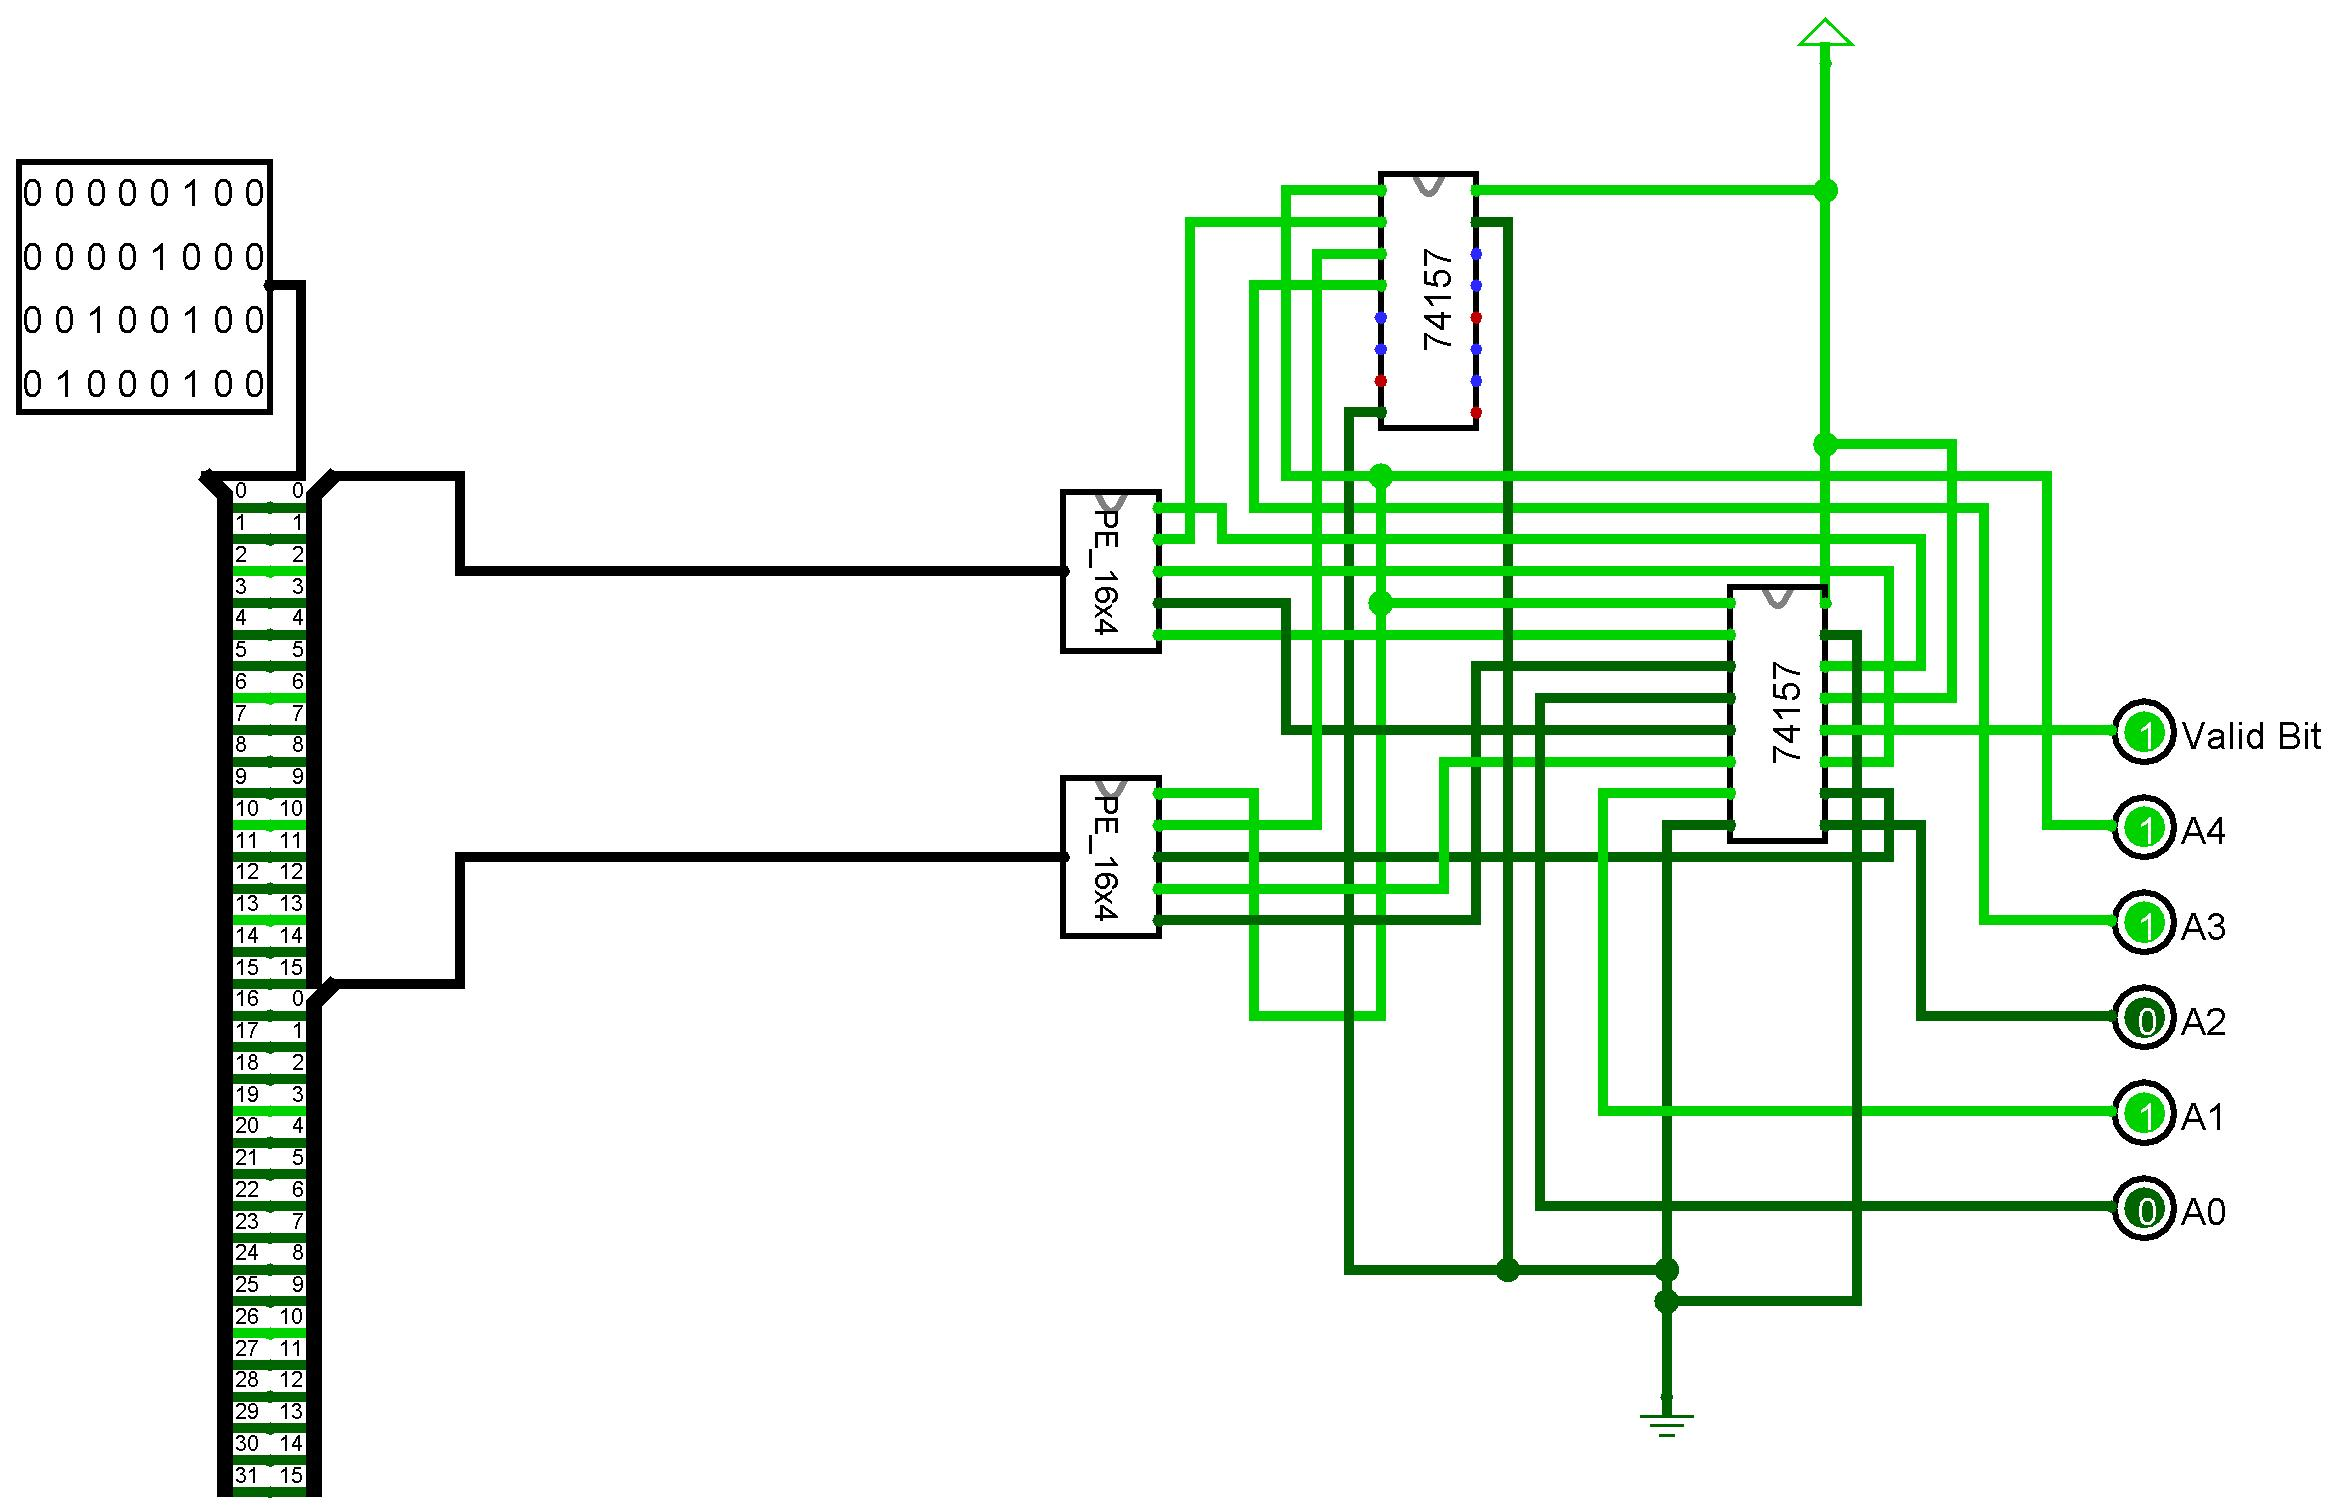
\includegraphics[width=\textwidth]{PE_32x5.jpg}
        \caption{32$\times$5 Priority Encoder}
        \label{fig:32x5prioenc}
    \end{subfigure}
    \caption{Encoder Circuits}\label{fig:encoder}
\end{figure}
\newpage
\subsection{Normalizer Circuit}
The normalizer circuit does necessary change in mantissa and exponent to change the number in operable form for other circuits.
\begin{figure}[H]
    \centering
        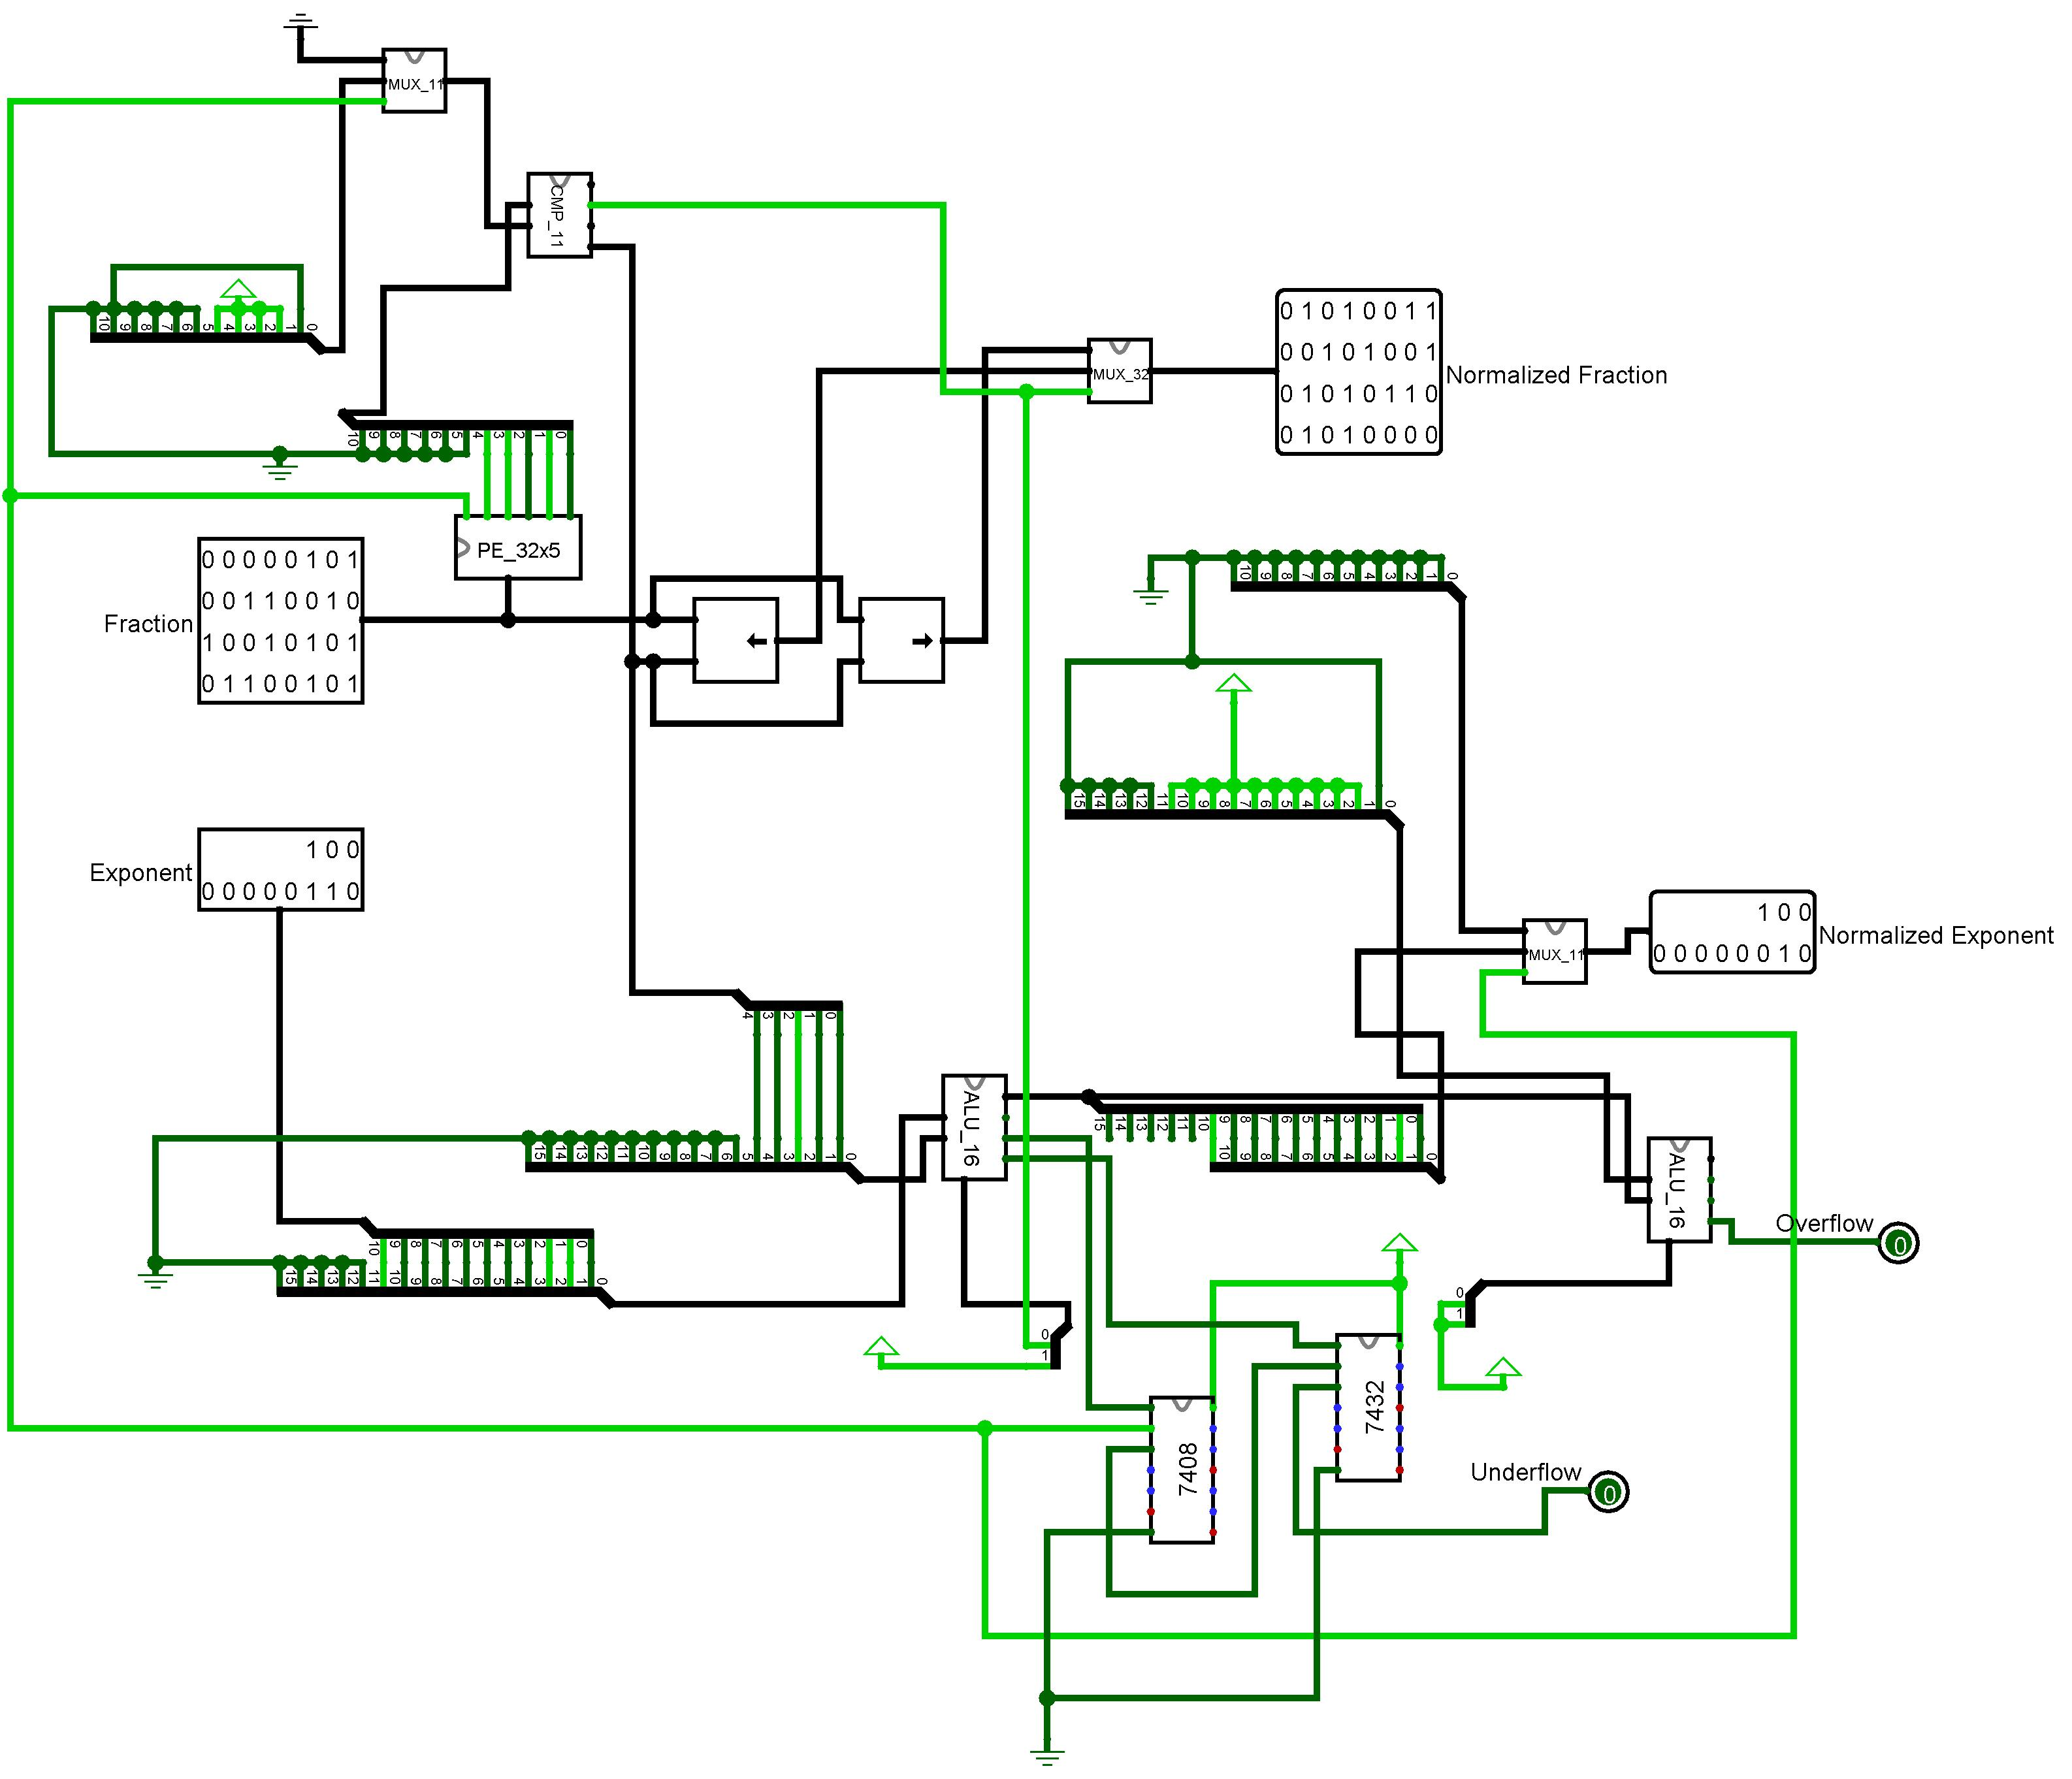
\includegraphics[width=\textwidth]{Normalizer.jpg}
    \caption{ Normalizer Circuit }\label{fig:normalizer}
\end{figure}


\newpage
\subsection{Rounder Circuit}
This circuit does the rounding of the mantissa in the result.
\begin{figure}[H]
    \centering
        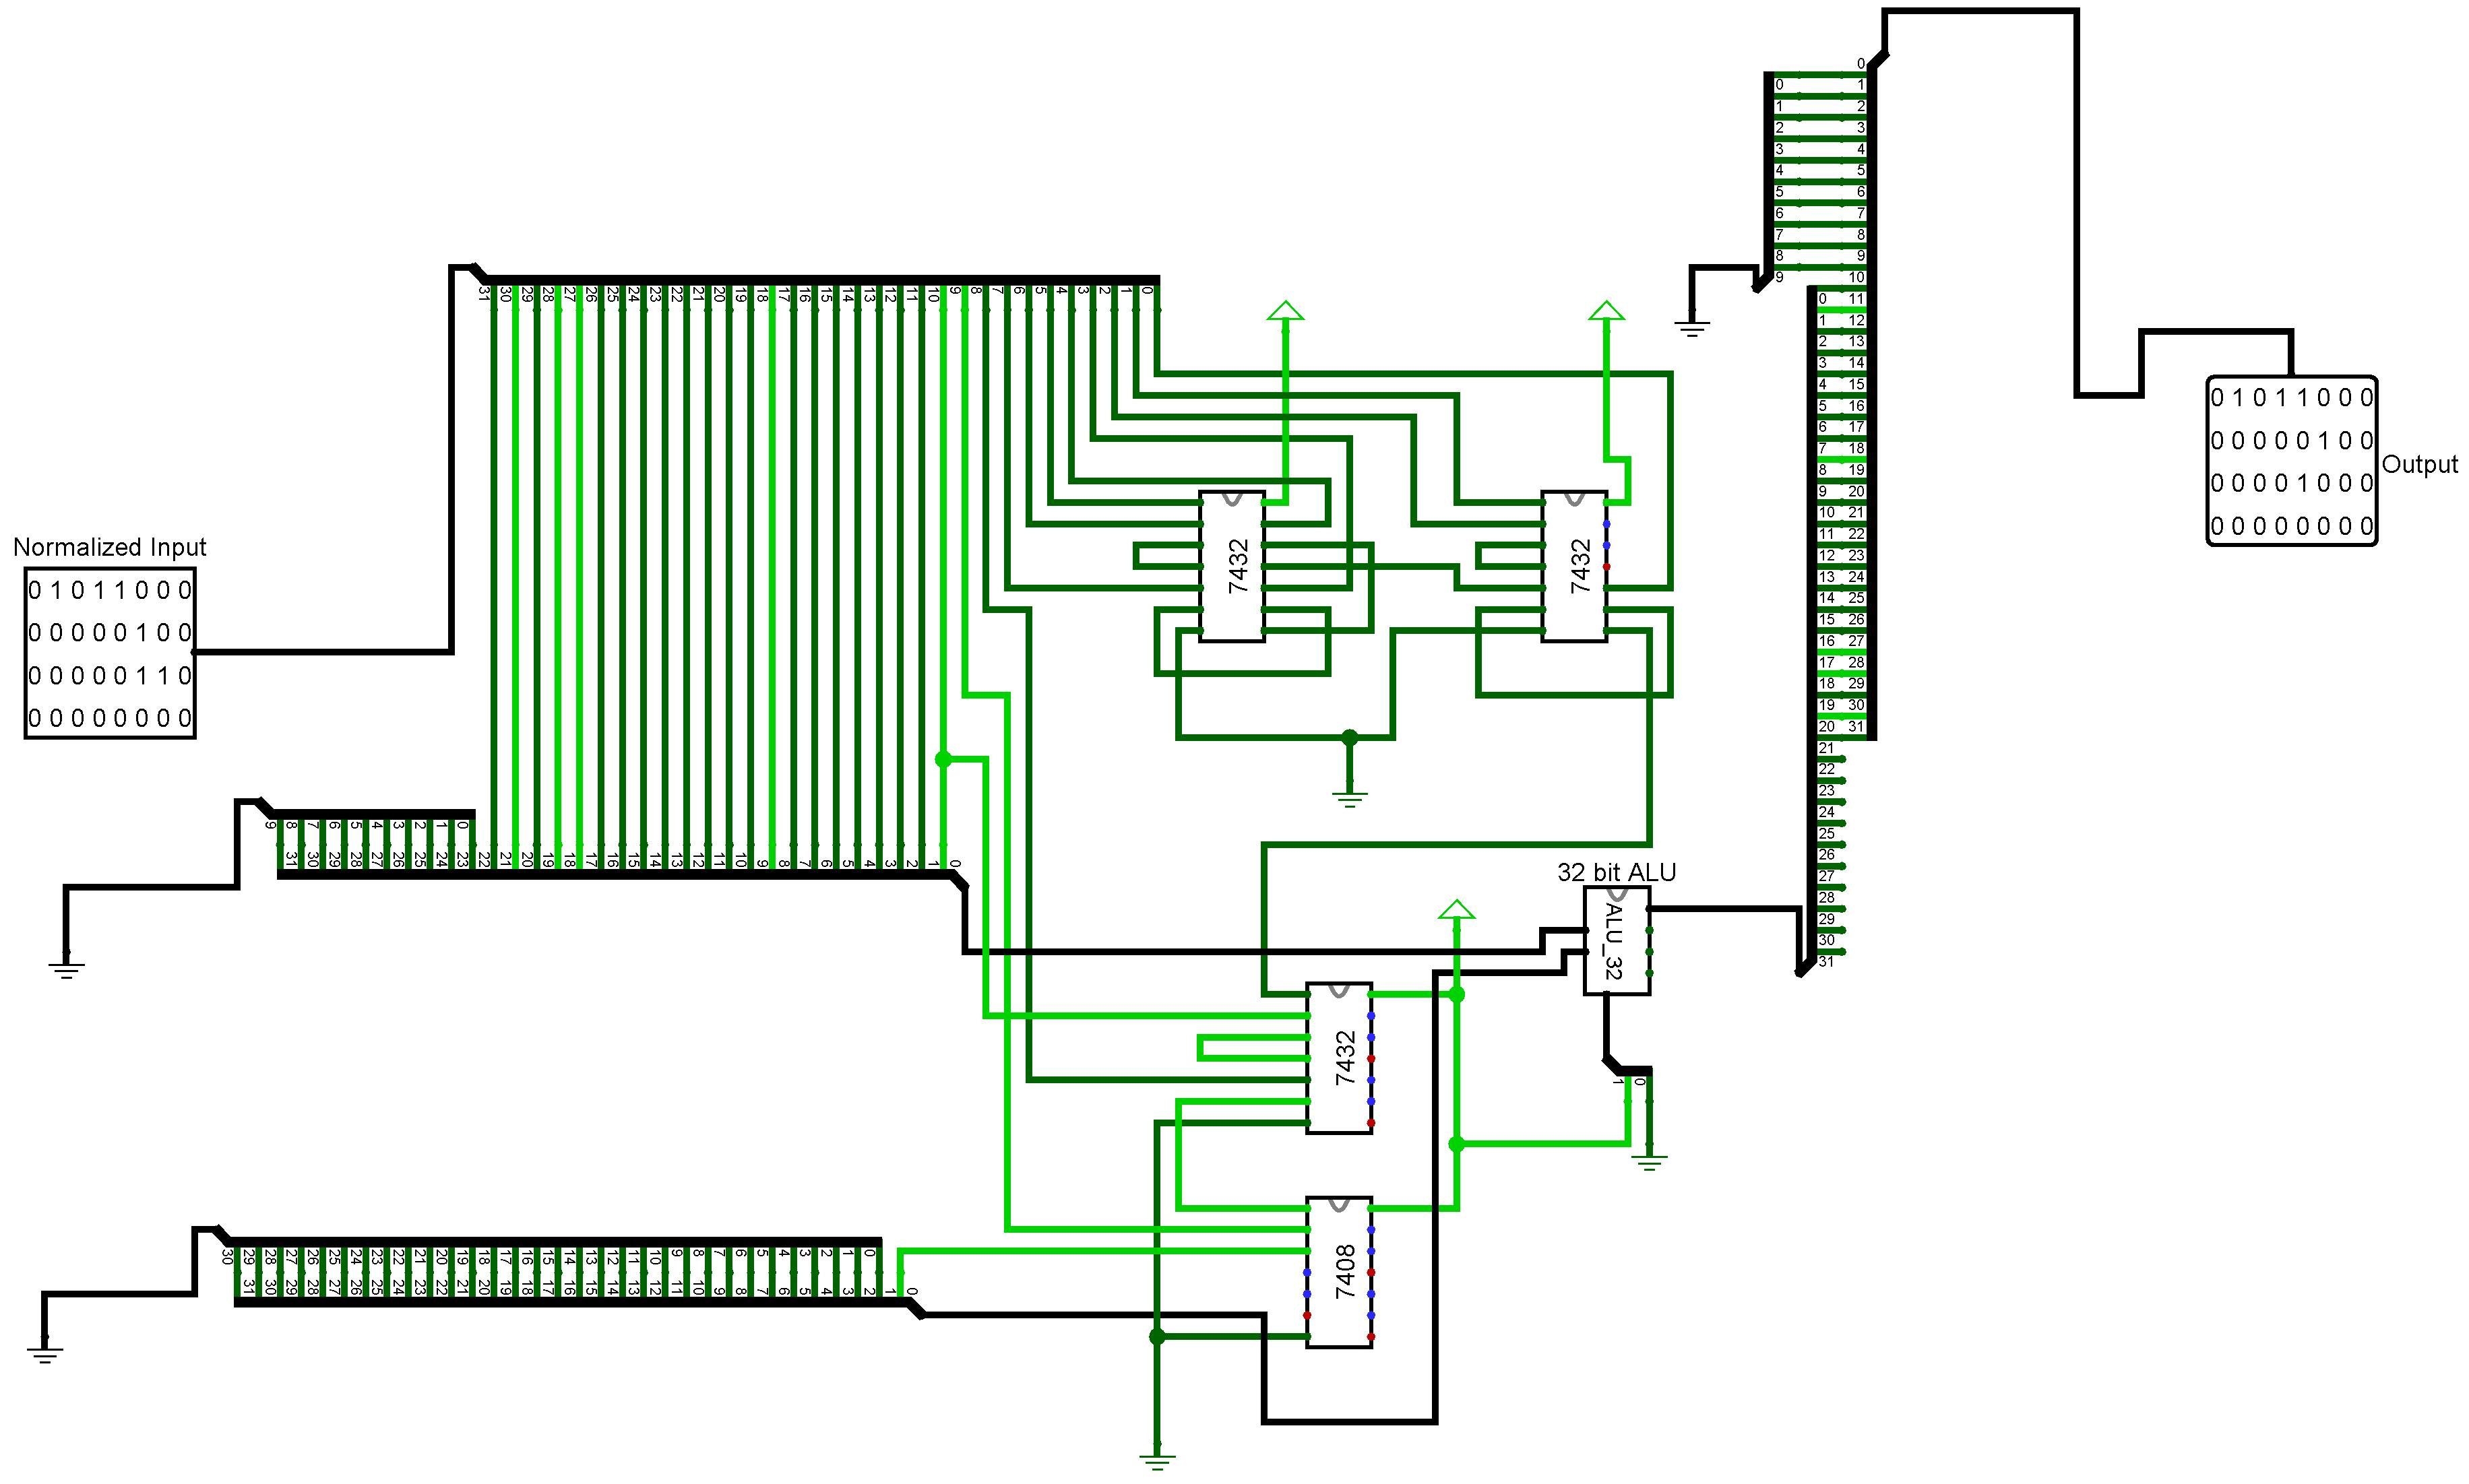
\includegraphics[width=\textwidth]{Rounder.jpg}
    \caption{Rounder}\label{fig:rounder}
\end{figure}

\subsection{Input Pre-processors}
This module validates the input given by user . It contains:
\begin{itemize}
    \item A Single Input Checker that shows the validity of a single floating point number input
    \item A Input Validator containing 2 single input checkers to validate the whole input
\end{itemize}
\begin{figure}[H]
\centering
  \begin{subfigure}[b]{\textwidth}
  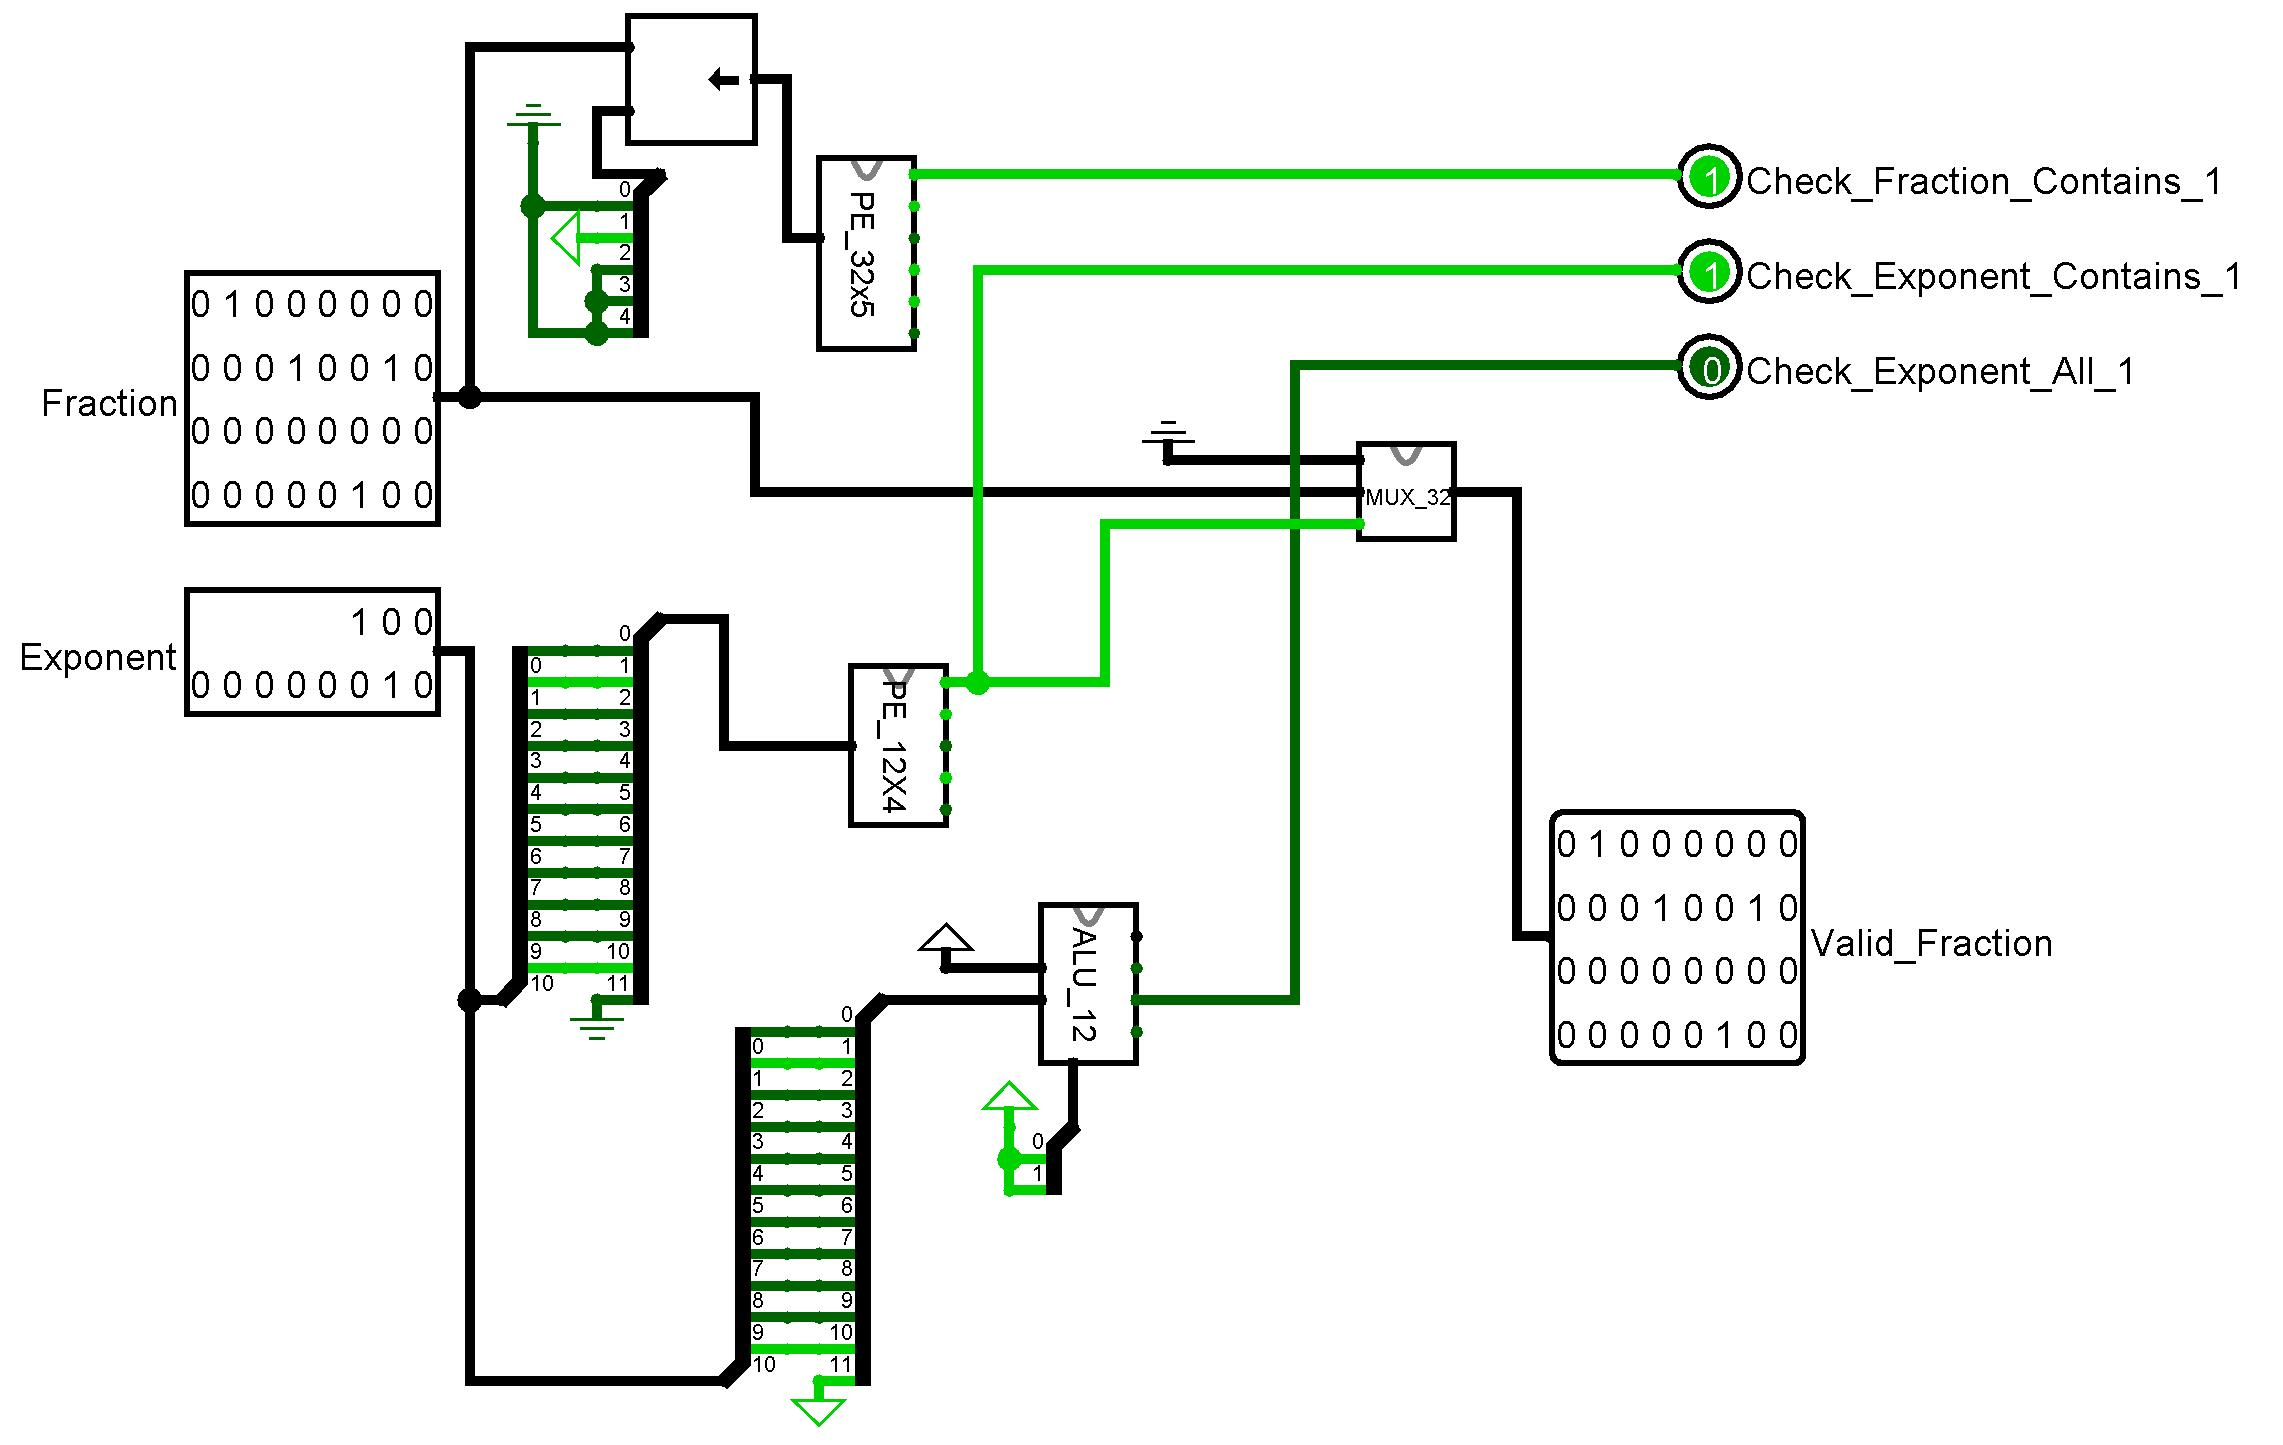
\includegraphics[width=\textwidth]{Single_Input_Checker.jpg}
  \caption{Single Input Checker}
  \label{fig:inpcheck}
  \end{subfigure}
  
 \begin{subfigure}[b]{\textwidth}
  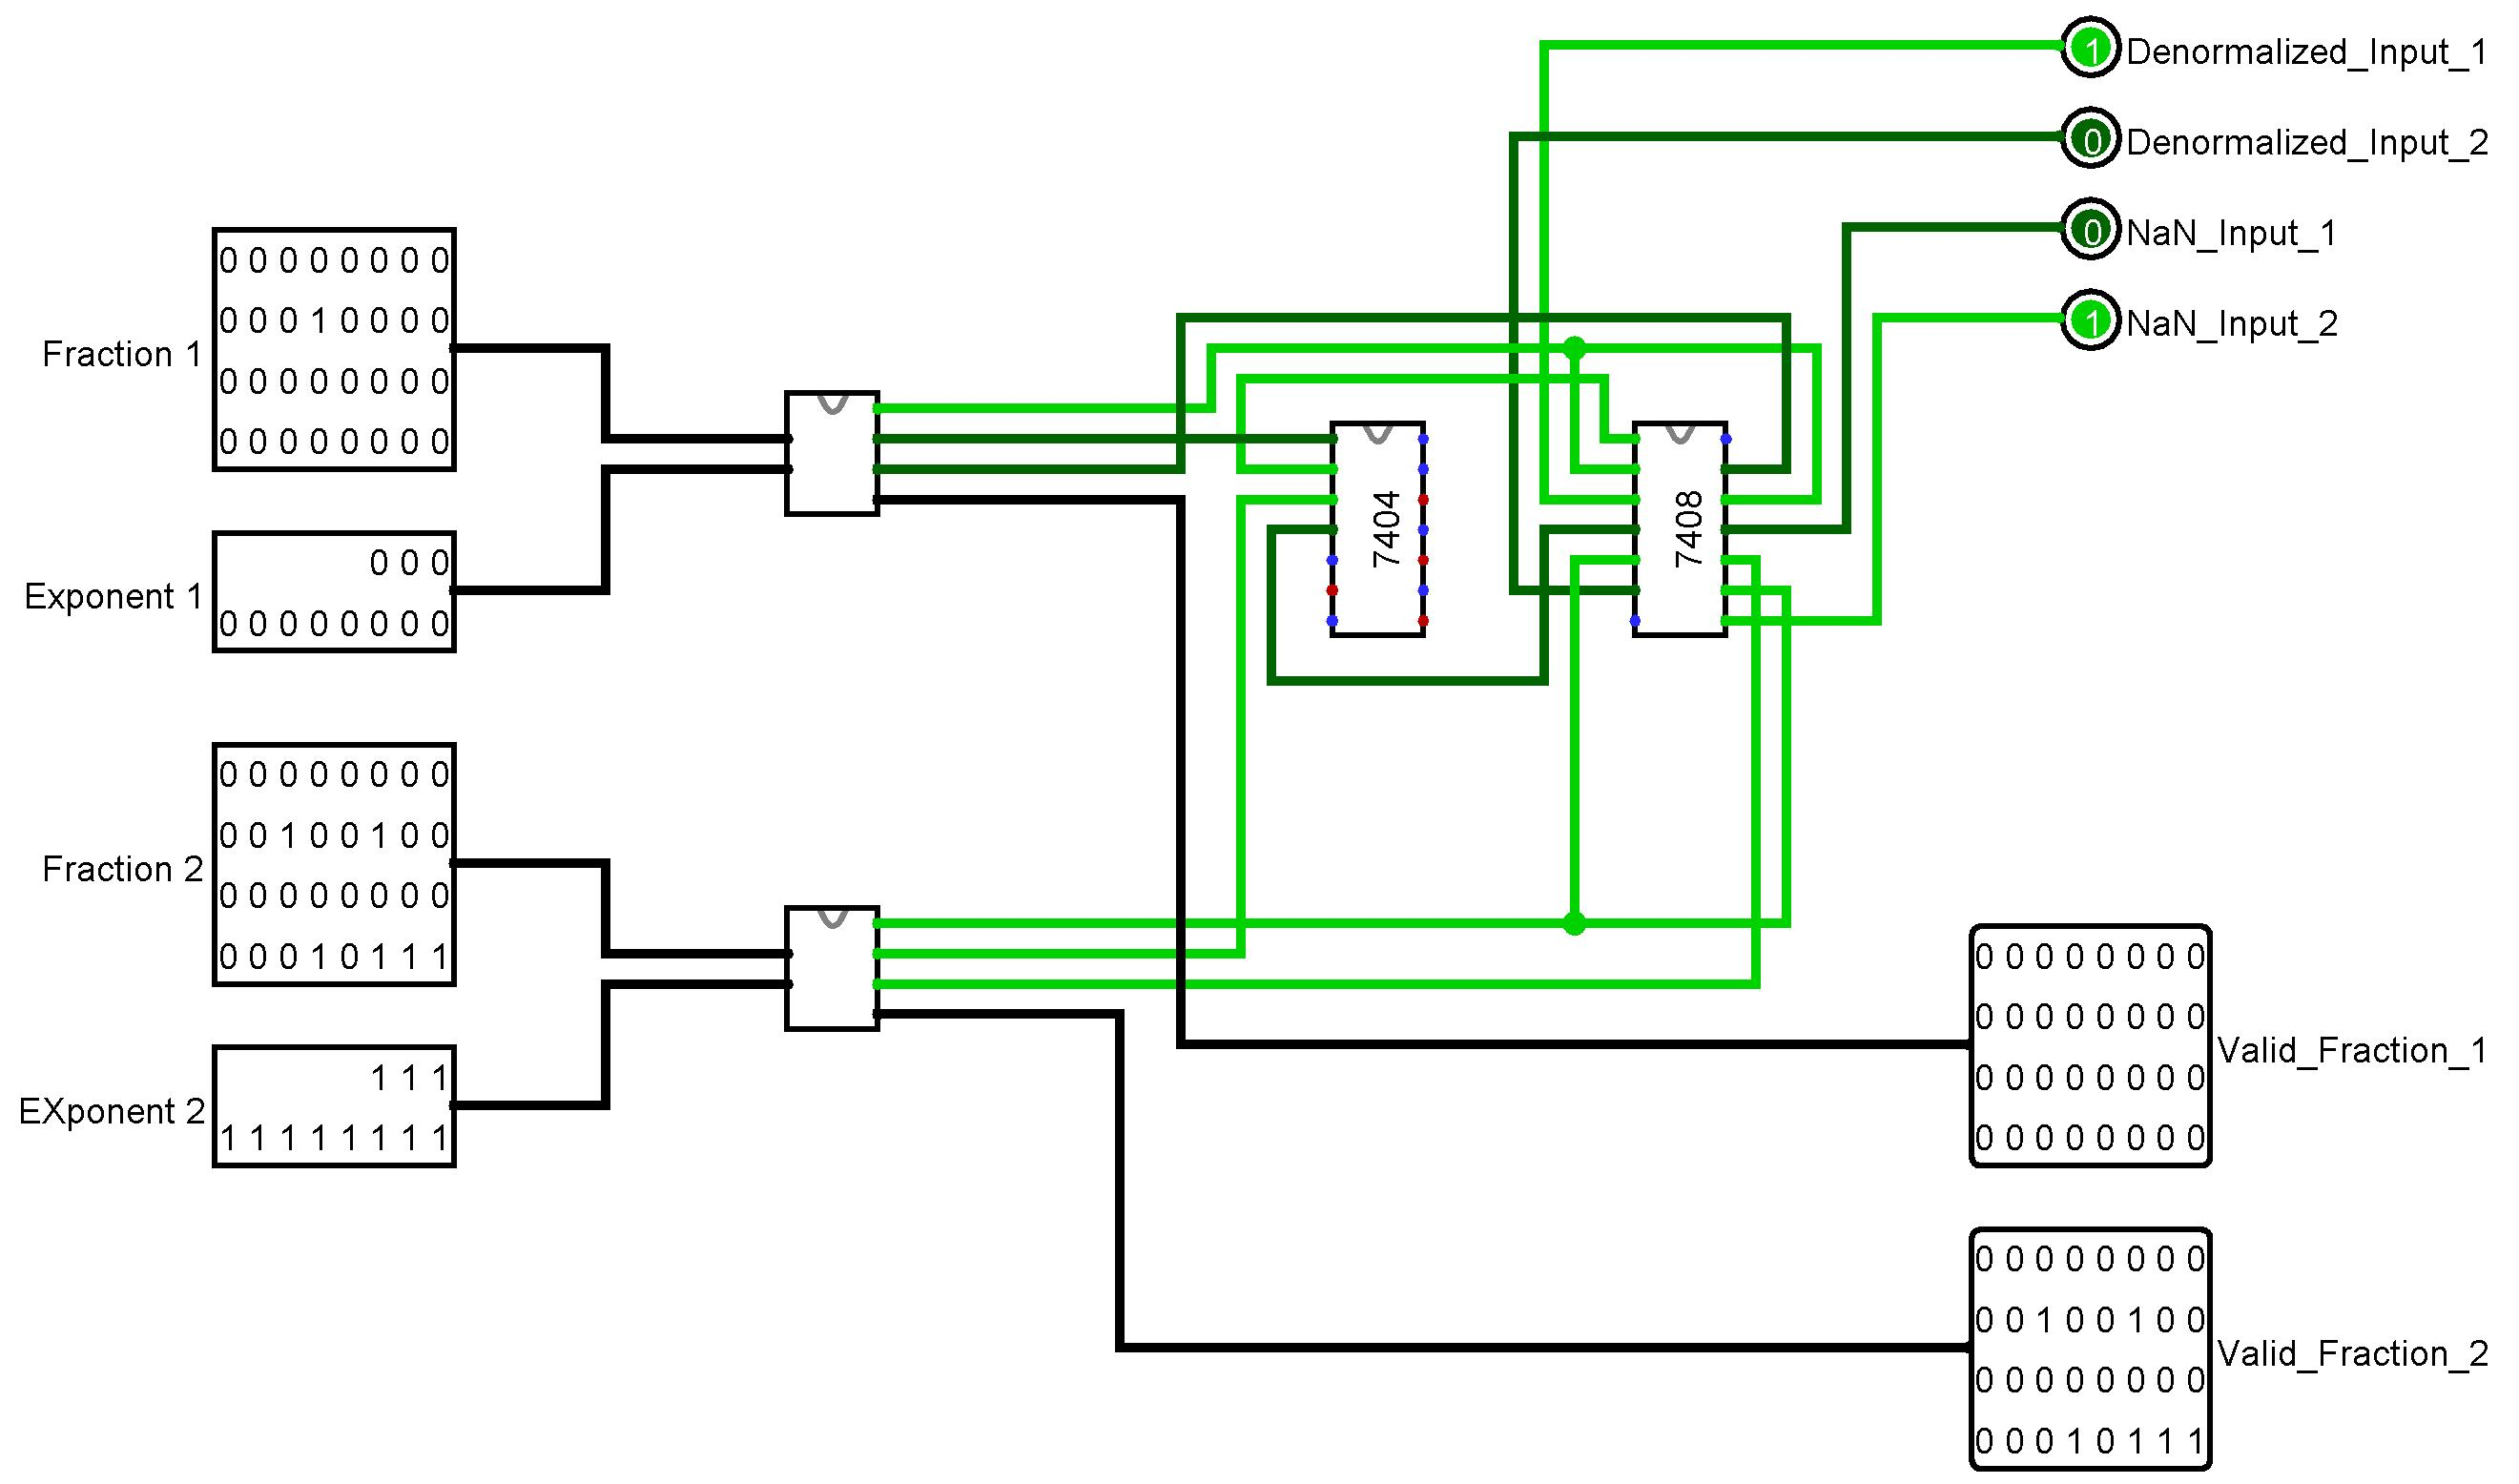
\includegraphics[width=\textwidth]{Input_Validator.jpg}
  \caption{Input Validator}
  \label{fig:inpval}
  \end{subfigure}
 \caption{Input Processing Utility}\label{fig:inpproc}
\end{figure}
\newpage
\subsection{ALU}
The 32 bit Arithmetic Logic Unit is used in several places in the circuit to perform add operation
\begin{figure}[H]
    \centering
    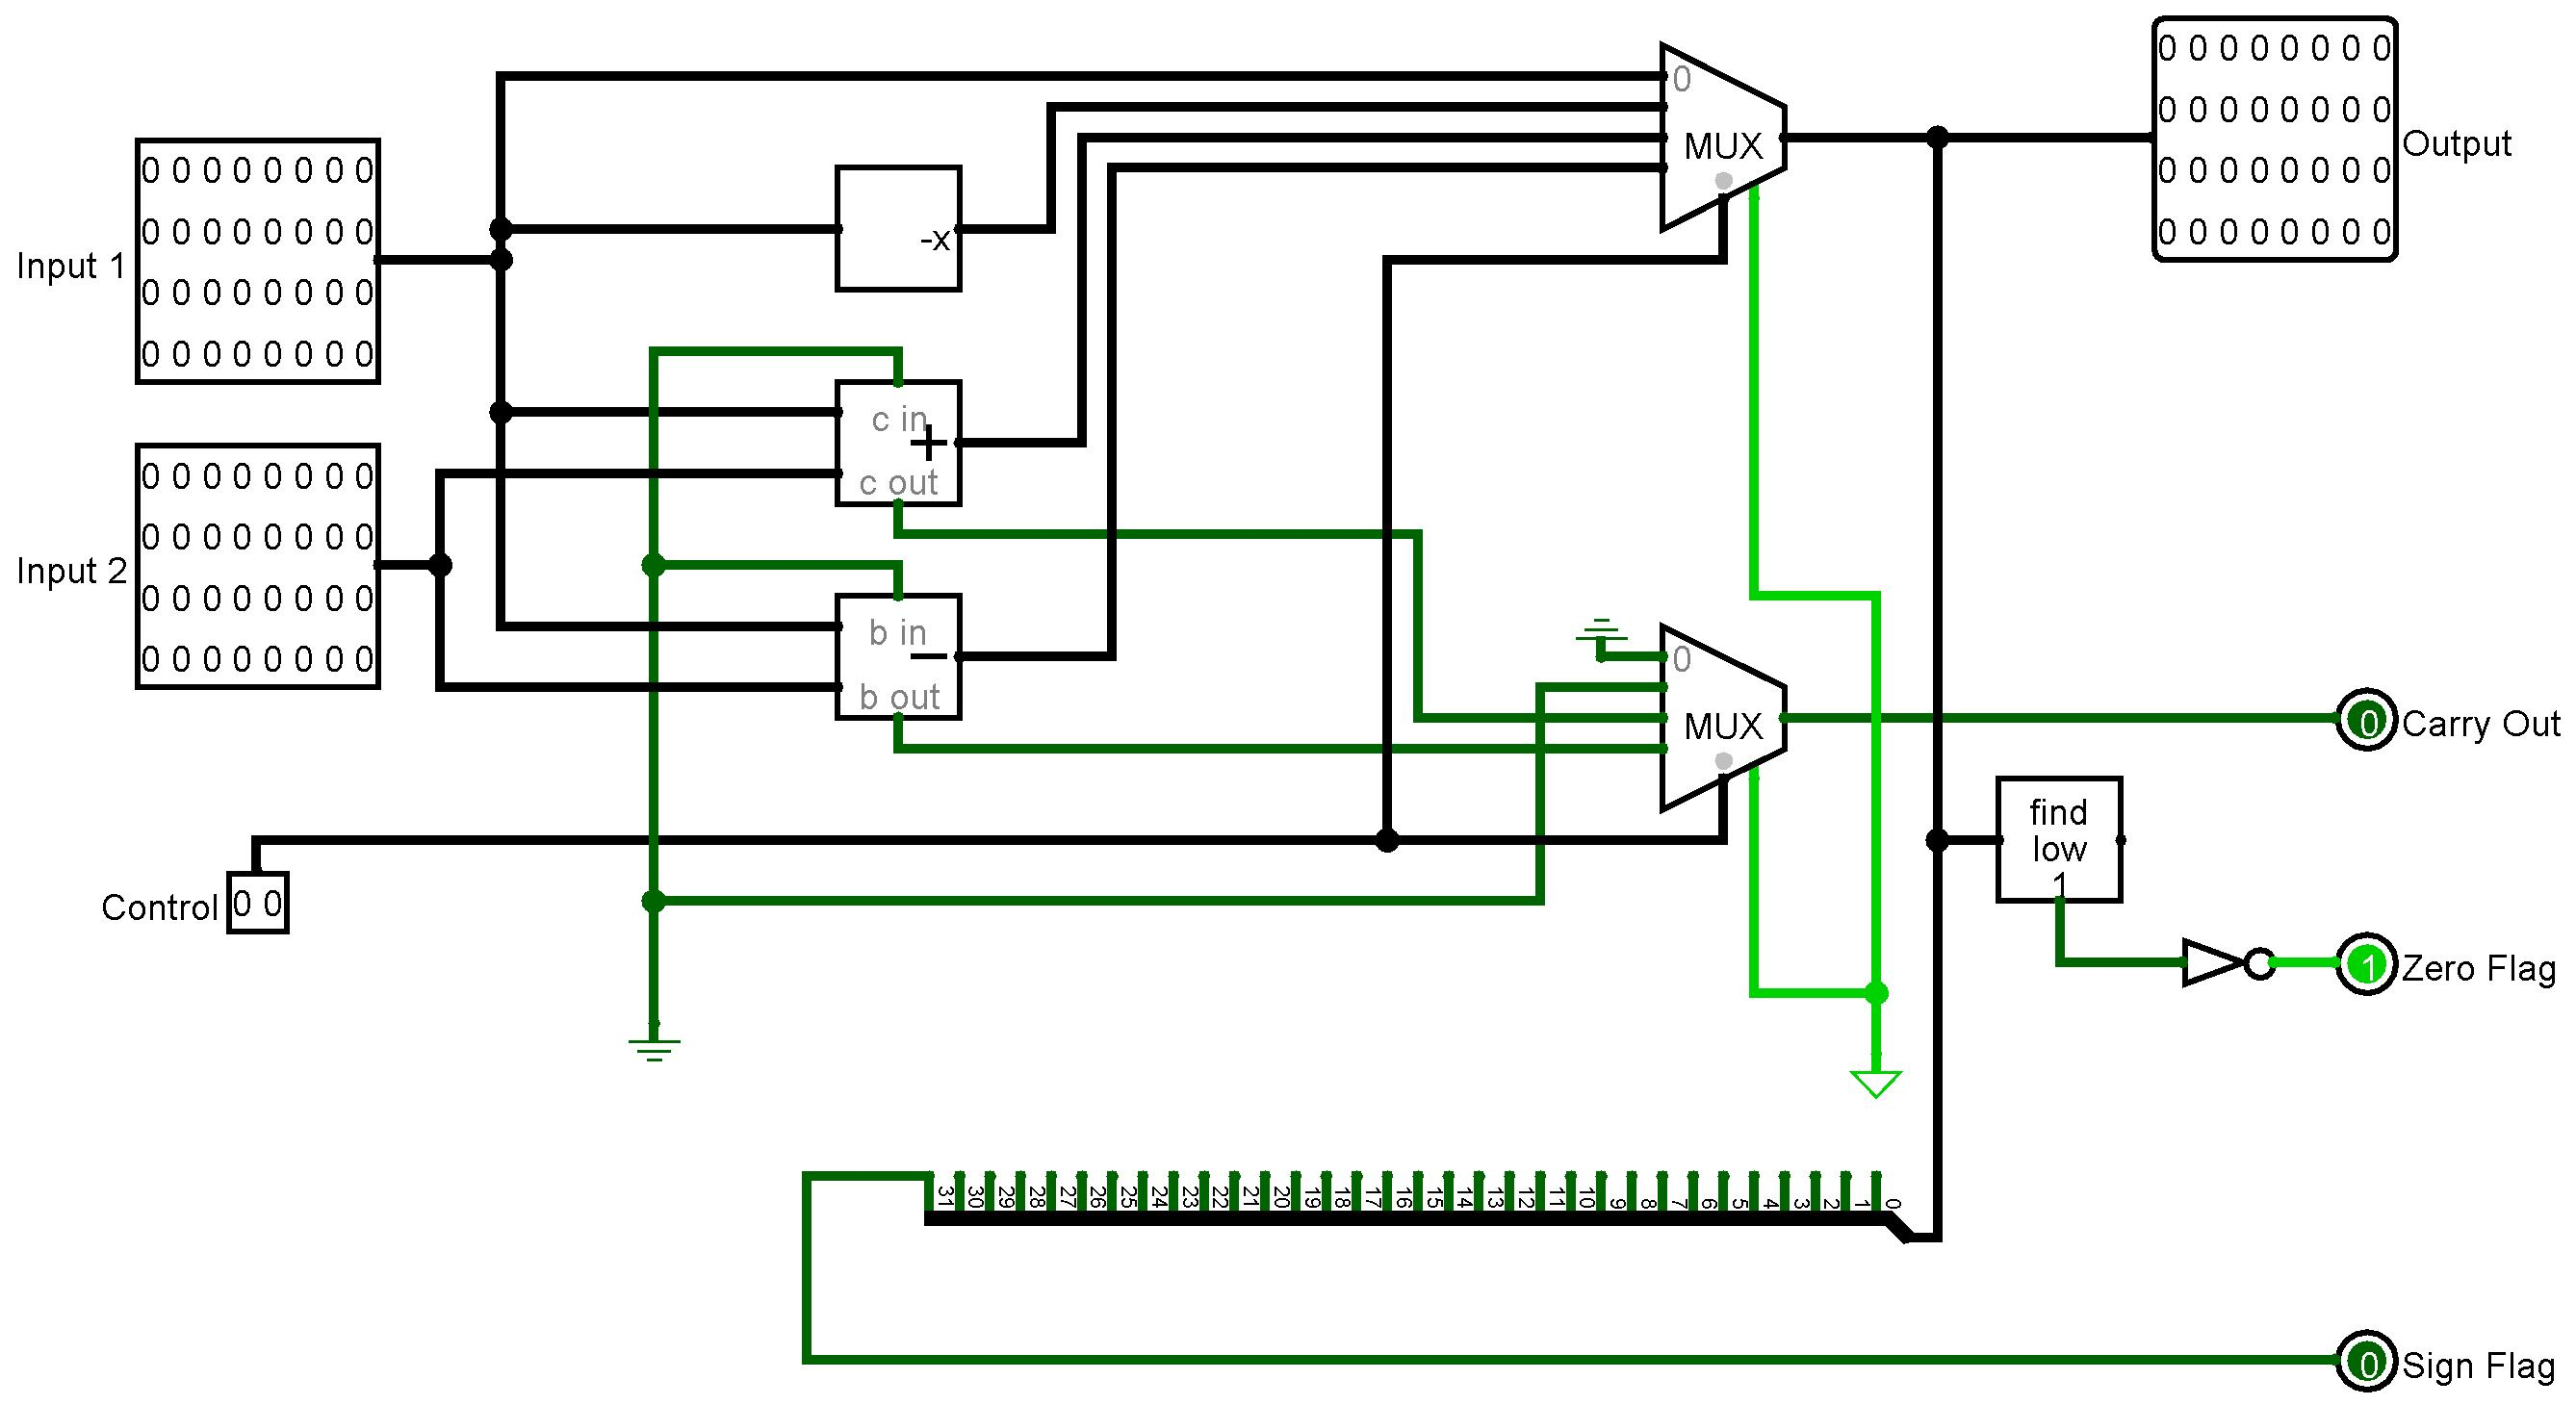
\includegraphics[width=0.7\textwidth]{ALU_32_bit.jpg}
    \caption{32 bit ALU}
    \label{fig:alu}
\end{figure}

\subsection{Floating Point Adder}
This is the actual floating point adder circuit which includes all the other libraries and circuits.
\begin{figure}[H]
    \centering
        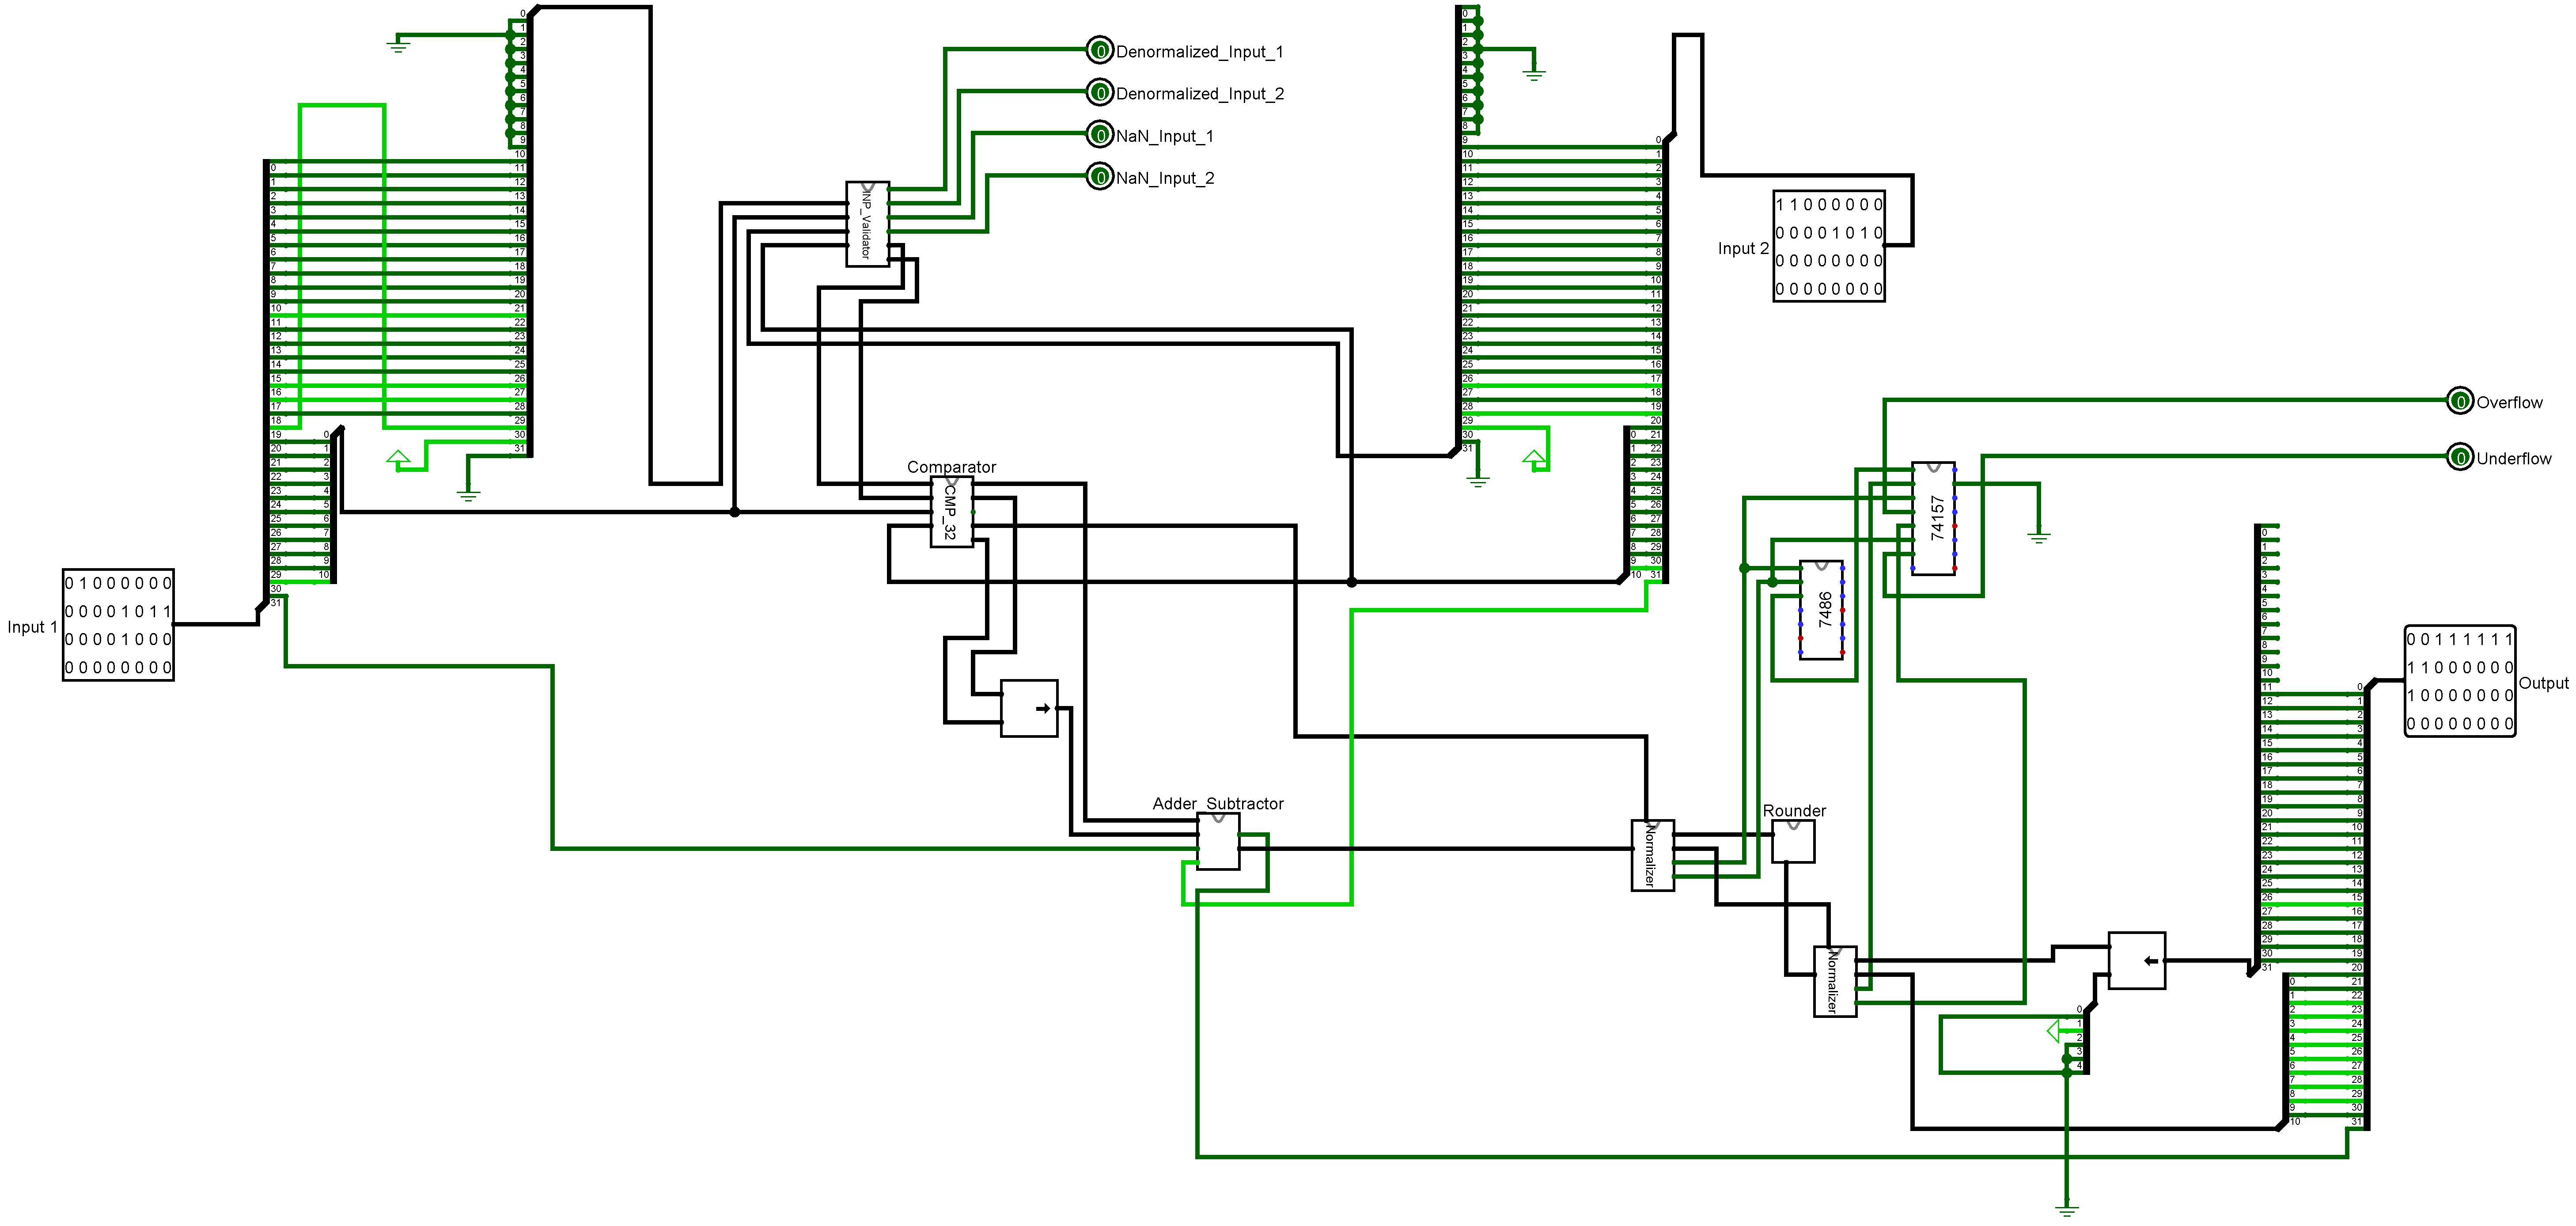
\includegraphics[width=\textwidth]{FPA.jpg}
    \caption{Floating Point Adder}\label{fig:fpa}
\end{figure}
\newpage
\subsection{Miscellaneous}
This is a circuit tester used for checking whether the output matches the desired answer or not. 
\begin{figure}[H]
    \centering
        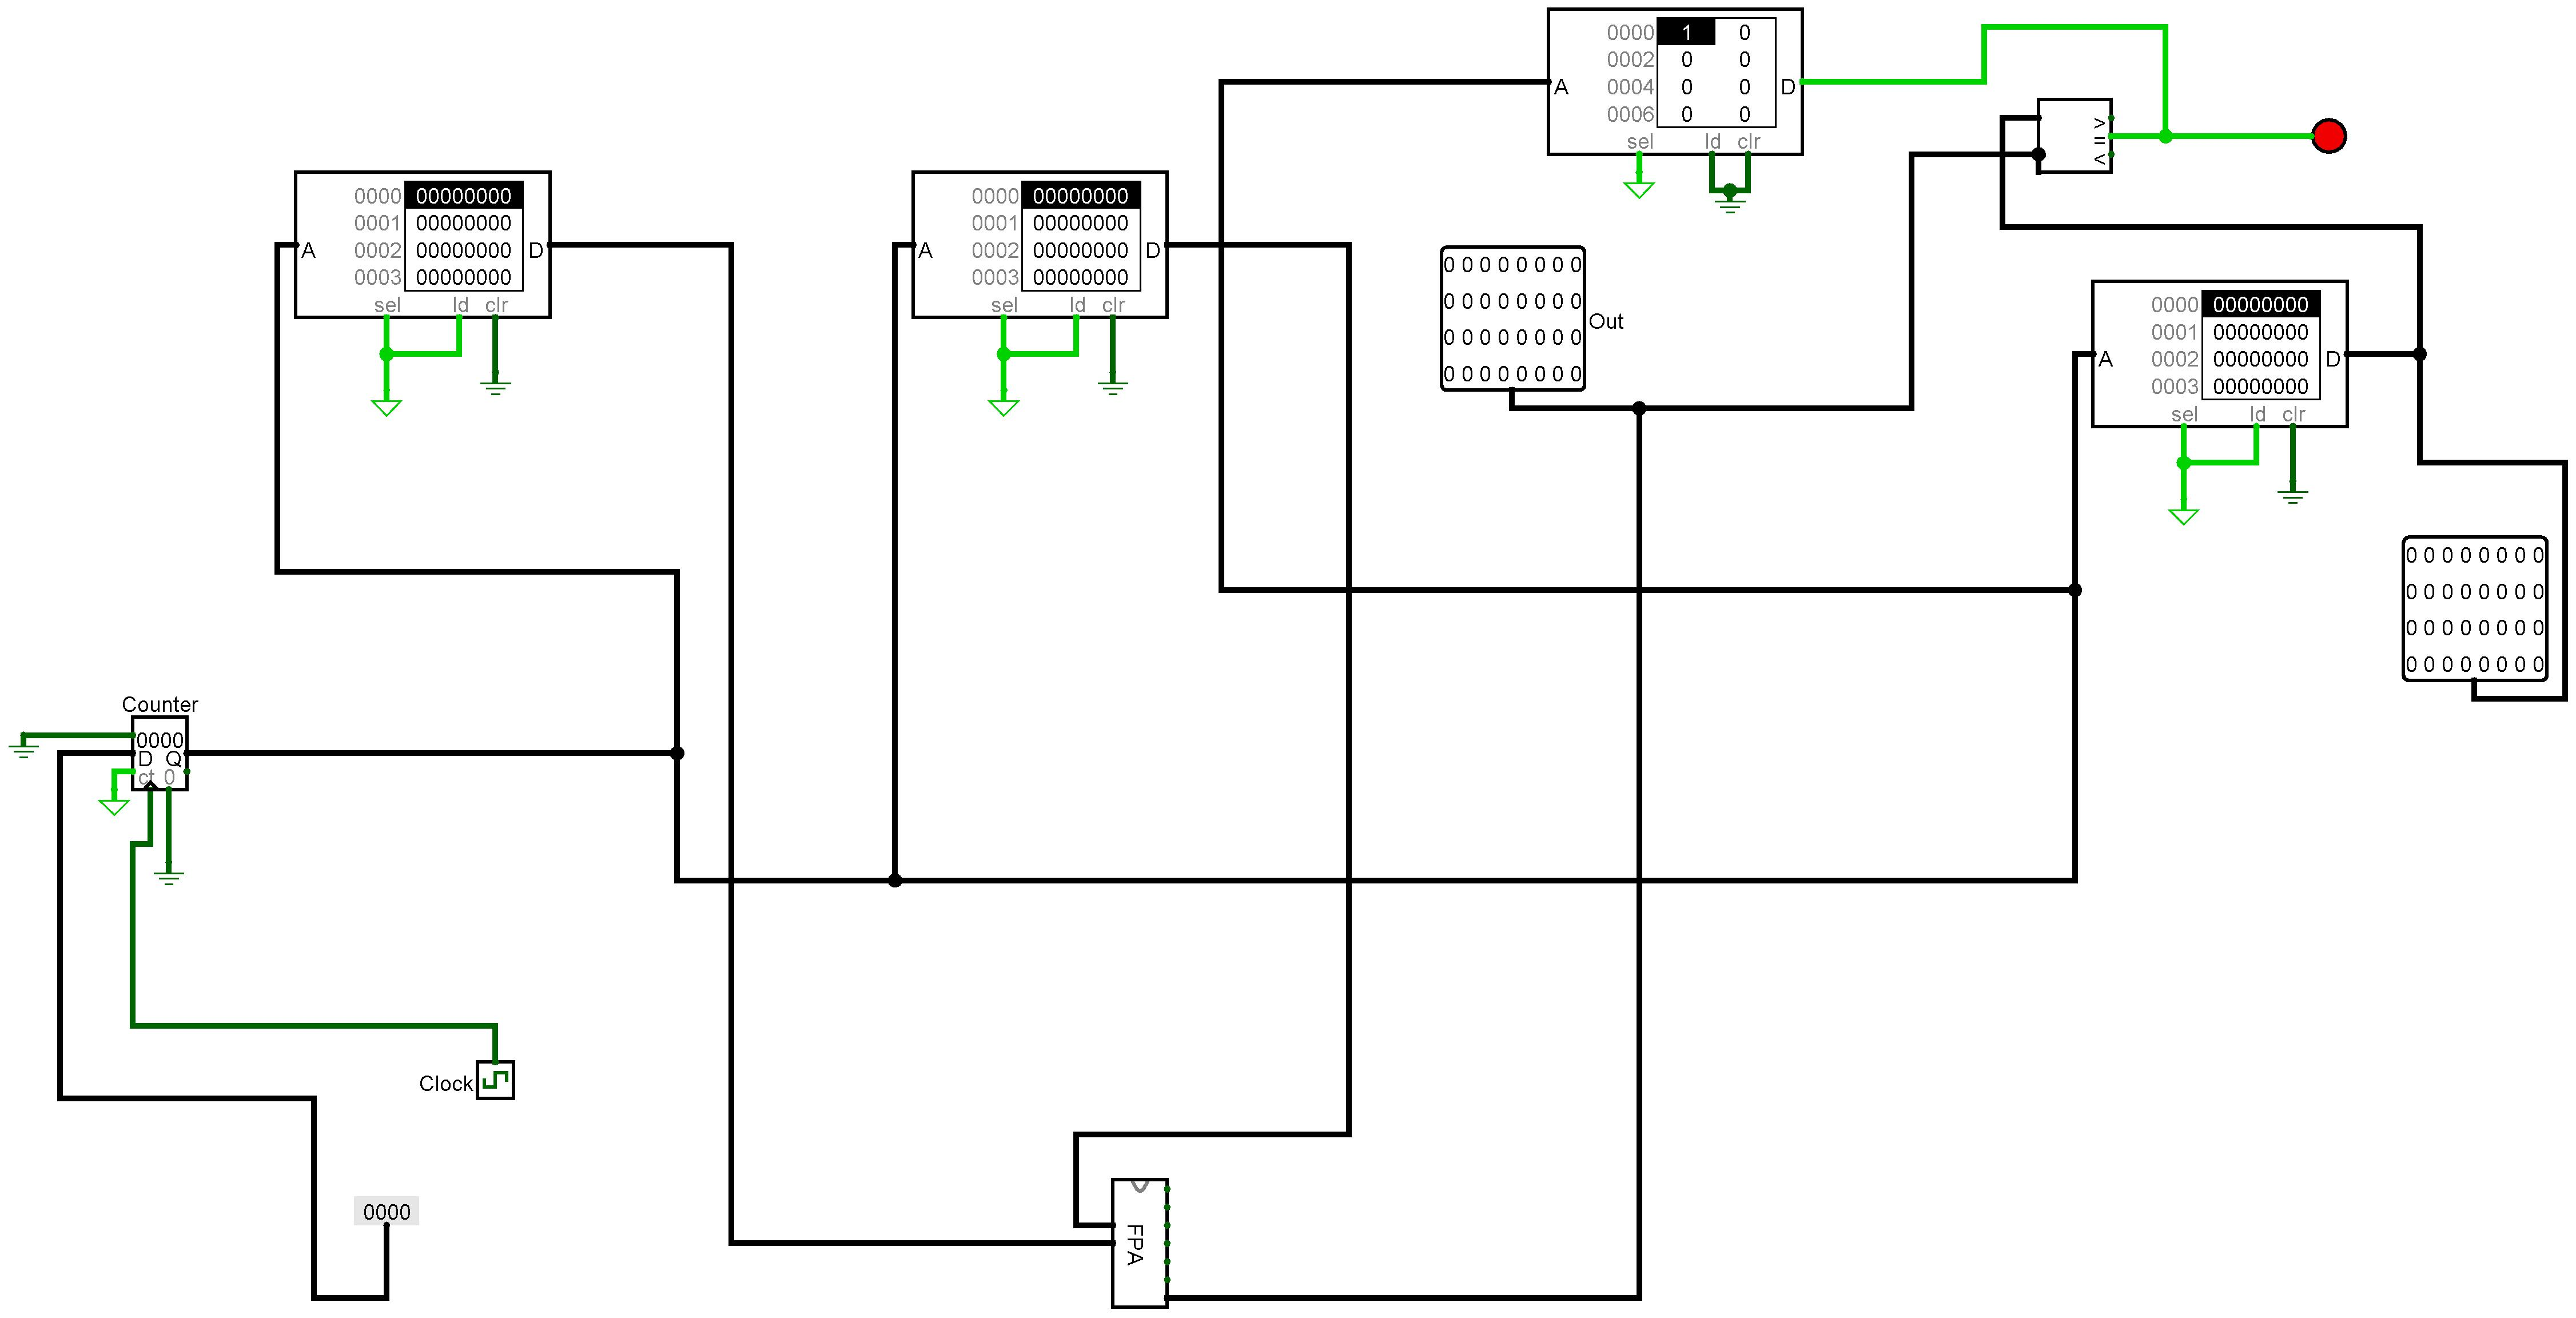
\includegraphics[width=\textwidth]{Circuit_Tester_Using_RAM.jpg}
    \caption{Circuit Tester}\label{fig:circtest}
\end{figure}
    
\end{document}
